
\chapter{The LHC and the CMS experiment}
%\epigraphfontsize{\small\itshape}
\epigraph{\itshape``You cannot swim for new horizons until you have courage to lose sight of the shore."}{--- \textup{William Faulkner}}


\label{ch:cms_experiment}
\section{Introduction}
\subsection{A new dawn}

\hspace{10pt}\lettrine[lines=2]{\initfamily{T}}{ he European Organization for Nuclear Research}, better known by its abbreviation "CERN", stands tall as a pillar of the human determination towards understanding nature. Paving the way for future collaborations by being one of the first examples of unity after the horrors of the past decade, CERN has been a home to experts coming from a multitude of fields ever since it opened its doors on the 29th of September 1954~\cite{History_CERN_1}. 

\hspace{10pt} Carefully positioned near Geneva (Switzerland), the newly formed institute had its eyes set on becoming the world's leading research facility for high energy physics. The following sections are going to briefly summarize the overall achievements of this collaboration which lead to the fulfilment of this goal and explain how bold decisions have resulted in the state of the art experiments operating at the moment. The easiest way to describe it would be to categorize the main benefits of CERN into three groups: scientific results, industry application and education.

 \hspace{10pt} Starting with the scientific achievements, the discovery of weak neutral currents~\cite{neutral_currents_1}\cite{neutral_currents_2} in 1973 made a huge breakthrough by confirming one of the basic ideas of the SM. Fast forward to ten years later when, after building from the previously gained experience, a new ground breaking result had been reported from CERN's experiments. It was the experimental evidence of the existence of W and Z bosons~\cite{WandZ_discovery}. Further technological advances combined with a non-conventional scientific strategy led to the design and the creation of the Large Electron-Positron (LEP) collider~\cite{LEP_TDR}. What followed was a series of high profile results, some of which will be discussed in the next section, that culminated with the creation of the Large Hadron Collider (LHC) and the subsequent discovery of the Higgs boson by the CMS and ATLAS experiments in 2012.

\hspace{10pt}Looking at the aforementioned discoveries one could naively assume that, while they represent a giant leap in our understanding of nature, nothing coming out of CERN's doors has a direct impact on everyday life. Yet this couldn't be further from the truth. It can easily be seen by looking at something that is today considered an essential tool in lives of many, the World Wide Web standard. Born in the dark corridors of building 1 within the research campus of CERN, the basis of our digital life had been created by Tim Berners-Lee~\cite{www_origins} in the early 90s for the purpose of easier data management within the experiments. This standard introduced the concept of associating Universal Resource Locators (URLs) to documents and other objects of interest as means of identifying and accessing them via internet. After being used internally for two years, it was concluded that the possible applications far exceeded its original goal and thus it was released to the public, setting a basis for what we now call web browsing.

\hspace{10pt}This general concern about the practicality of published results plagues not only high energy physics but also many of the fundamental branches of science. This constant questioning is even more baffling due to the fact that if only a minuscule investigative effort was made by those who present such claims, then it would be clear that many of technological leaps were enabled through fundamental research. Moving from the real of the internet, additional examples of this can also be found in medicine where the contribution of accelerator sciences are ranging from hadron therapies, which provide a less invasive way of treating cancer cells, to the development of super absorbent polymers for the purpose of creating thin but still multi layered baby diapers. As it would be touched on in the following sections, there are also going to be further industry applications of standards developed for the purposes of CERN experiments (but more about that in Section~\ref{sec:data_acquisition}).

\hspace{10pt} Finally, there is one additional way in which CERN impacts our society as a whole and that is through its education platform. Its main purpose is to give new generations of students the opportunity to participate in various programs that range form high school projects to undergraduate internship positions. This approach has influenced a large number of young people from all over the world to get involved in this field from a fairly early age. Case in point, the author of this thesis began his journey into the field of particle physics with his high school graduation thesis by looking into a set of simulation samples for a four muon decay of the, then still theorised, Higgs boson. Even though it was a fairly simple project, it was still a harbinger of a, hopefully long, future research career.

\subsection{Down the road less travelled}
\hspace{10pt} As a good rule of thumb, the high energy physics (HEP) scientific community organizes meetings and workshops every few years in order to encourage the discussion regarding future experiments. This should come as no surprise as planning ahead and trying to see the bigger picture represent actions closely associated with almost every successful long term venture. The need for this approach became more evident in the decade that saw the experimental confirmation of the existence of the neutral current and the discovery of W and Z boson, as it became clear that there is an urgency for a structure that could probe the, then freshly finalized, Standard Model.

\hspace{10pt} The decision to move away from proton-antiproton machines, for which CERN had developed expertise in the past decade, in favour of an electron positron design had a much bigger impact on the institute (and HEP community as a whole) than it was initially envisioned. From a strictly physics point of view, this opened the door to a much cleaner slate that enabled detailed probing of the electroweak sector. On the other hand, taking a look at the engineering and monetary side, a circular collider being built under Geneva had pretty much set in stone the future of Europe's particle physics strategy. The grandiose projects being discussed in USA (the Superconducting Super Collider~\cite{SSC_proposal}) and Russia (the proton Accelerating and Storage Complex - UNK~\cite{UNK_proposal}), some of which were promising center of mass energies much larger than those achieved by the LHC today (altough with much less total projected luminosity), were halted and ultimately cancelled due to budgetary and political constrains. It should come as no surprise that one of the main reasons for the success of the LHC project was the fact that it re-uses the same tunnel that was built years ago for LEP.

\hspace{10pt} The construction of the tunnel turned out to be one of the biggest civil engineering achievement in Europe at the time. The completion of the, 27~km in circumference, home of the accelerator complex was done in 1988 after a five year effort. Time for proper celebration came one year later, when the first beams were collided in August of 1989. Following the planned scientific program, the first item on the agenda was to probe Z bosons, which is why the starting beams each bore the energy of $45$~GeV, thus matching the boson's mass in the center of mass frame. Following in the same vein, the next interest was to take the total energy higher, leading it to the the WW production range. It required an upgrade of the accelerator, resulting in the increase in energy to $100$~GeV per beam. The limit beam energy of the machine reached $209~$GeV near the end of its operation period. At the same time a possible appearance of the Higgs boson-like particle was looming over the planned end date of LEP and the beginning of LHC's construction.

\hspace{10pt} At the time thought of as a possible swan song of LEP, a 91~\% confidence level (or 1.7$~\sigma$) indication of an excess at around $115~$GeV was reported by researchers in early year 2000. Prompted by this information, an extension of a couple of months was approved in order to further explore this appearance. Unfortunately for researchers, this time didn't yield any significant improvement and LEP was shut down by the end of the year, leaving a sense of a lost opportunity in the eyes of many~\cite{LEP_searches}. All the subsequent arguments of a biased decision making were confirmed to be void when the $125~$GeV Higgs boson was discovered by the CMS and ATLAS experiments.


\subsection{The Machine}
\hspace{10pt} The successor to LEP, the Large Hardon Collider (LHC)~\cite{LHC_TDR}, originated with the idea of further testing the phase space of high energy physics. Commonly nicknamed the "Higgs discovery machine", it was designed with a much broader physics program. Representing a natural evolution from the previous generation, this machine was built to collide protons at very high energies ranging from 7 until 14~TeV (in the centre of mass frame).

\begin{figure}[htbp]
  \centering
    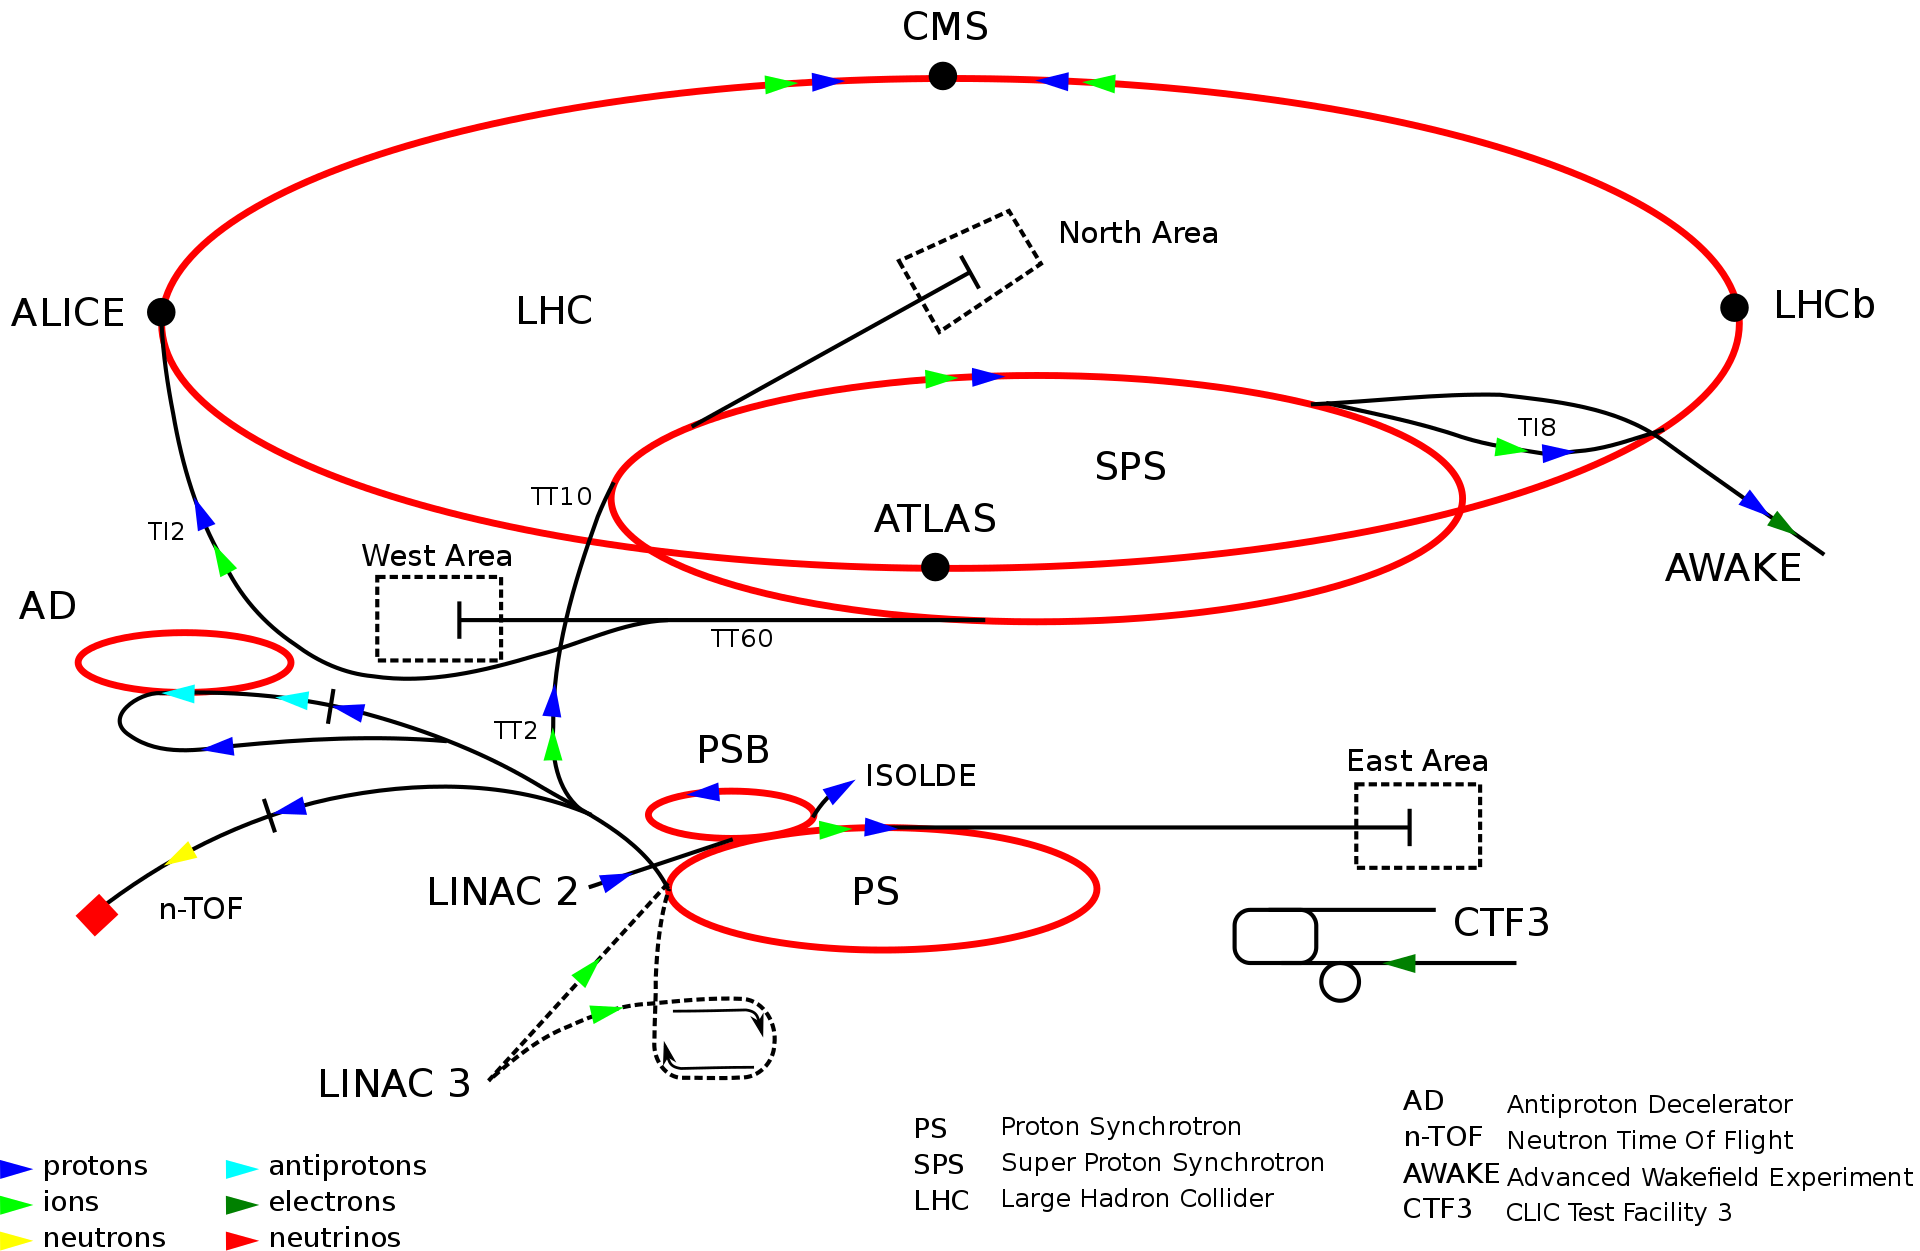
\includegraphics[width=0.8\textwidth]{CMS_experiment/LHC.png}
  \caption[Schematic representation of the LHC complex.]{Schematic representation of the LHC complex.}
  \label{fig:lhc}
\end{figure}

\hspace{10pt} The diversity of research areas covered by the LHC can best be seen in by looking at the coverage achieved by main experiments residing at four beam intersection points. Two general purpose experiments, ATLAS and CMS, take the center stage by being the main reason for the LHC's nickname. Adding the heavy ion research to the list, the ALICE experiment\footnote{With a help from the CMS experiment} takes the role of a primary experiment in within the field~\cite{ALICE_paper}. Finally, the LHCb experiment~\cite{LHCb_paper} proved crucial to the research ideas involving heavy flavour physics.

\hspace{10pt} The journey of a proton bunch begins with a canister of hydrogen gas, whose atoms are stripped from electrons by using an electric filed while the remaining protons are being passed on to the first step of acceleration - CERN's Linear Accelerator 2 (LINAC 2). Bringing the energy of particles to 50 MeV, it passes them on to the second step, the Proton Synchrotron Booster (PSB).  It further increases the energy of the particles reaching the values of 1.4 GeV before continuing towards the Proton Synchrotron (PS), where bunches reach the energies of 25 GeV. The final step in this process is the Super Proton Synchrotron (SPS) which brings the increase in energy to a total of 540 GeV. After this, particles are finally reaching the LHC, where their energy is further increased to a more desirable range of 7-14~TeV.


\hspace{10pt} The status of the LHC operation is best described when separated into three parts. During the writing of this thesis these could've been defined as the past, present and future of collider physics. Ranging from the period of 2009 to 2013, the past is manifested in the form of the Run 1 phase of operation. Colliding beams at 7 (and 8) TeV, the first cycle of operation brought in around $27~\text{fb}^{-1}$ of collected data, when looking from the CMS experiment's point of view. The beginning of this era was marked with a more than a year long delay, due to damage caused by an unexpected magnet quench. After the mandatory stop the journey was continued, first conservatively, by reaching energies of $1.18$~TeV per beam. This was enough to beat the previous record held by Tevatron collider (Fermilab)~\cite{tevatron_summary} and to put a first check on LHC's goal list. Increases in operational energy continued starting with $3.5~$TeV in 2010 and continuing in 2012, when the energy was set to $4$~TeV per beam marking the maximum reached during this stage. The most important achievement of this era (or better to say till this day) was the discovery of the Higgs boson in July of 2012. In order to be better prepared for the next stage, the LHC went into a shutdown period in 2013. 

\hspace{10pt} The first collision of $6.5~$TeV beams achieved on the 20th May of 2015 sounded the beginning of the current, Run 2, era of operation. Starting with the summer of 2016, the LHC reached its designed luminosity of $1.0\cdot10^{34}$~cm$^2$s$^{-1}$ (increasing it to twice the value before the shutdown). Brining in the total of $\sim130~$ fb$^{-1}$, Run 2 phase creates opportunities for precision measurements and probing of the BSM phase space (at the very least, excluding parts of it). Detector upgrades, some of which are going to be discussed in the following sections, brought a more efficient way of selecting relevant data by inserting complex, mode targeting selections early during triggering process. Currently, LHC experiments are working towards publishing a multitude of "legacy" results that are going to summarise and publicly release the conclusions made during this phase of operation.

\hspace{10pt} The future begins with the Run 3 phase of operation, which is expected to bring new ways of selecting data. Applying industry standard Machine Learning (ML) algorithms for research purposes, newly created triggers are expected to bring a significant increase in sensitivity for many of the BSM searches. Following this period, another upgrade stage is set to take place in order to prepare the machine for the next big step - the High Luminosity LHC. Figure~\ref{fig:lhc} showcases the LHC operation timeline with the projected integrated luminosity. 

\begin{figure}[htbp]
  \centering
    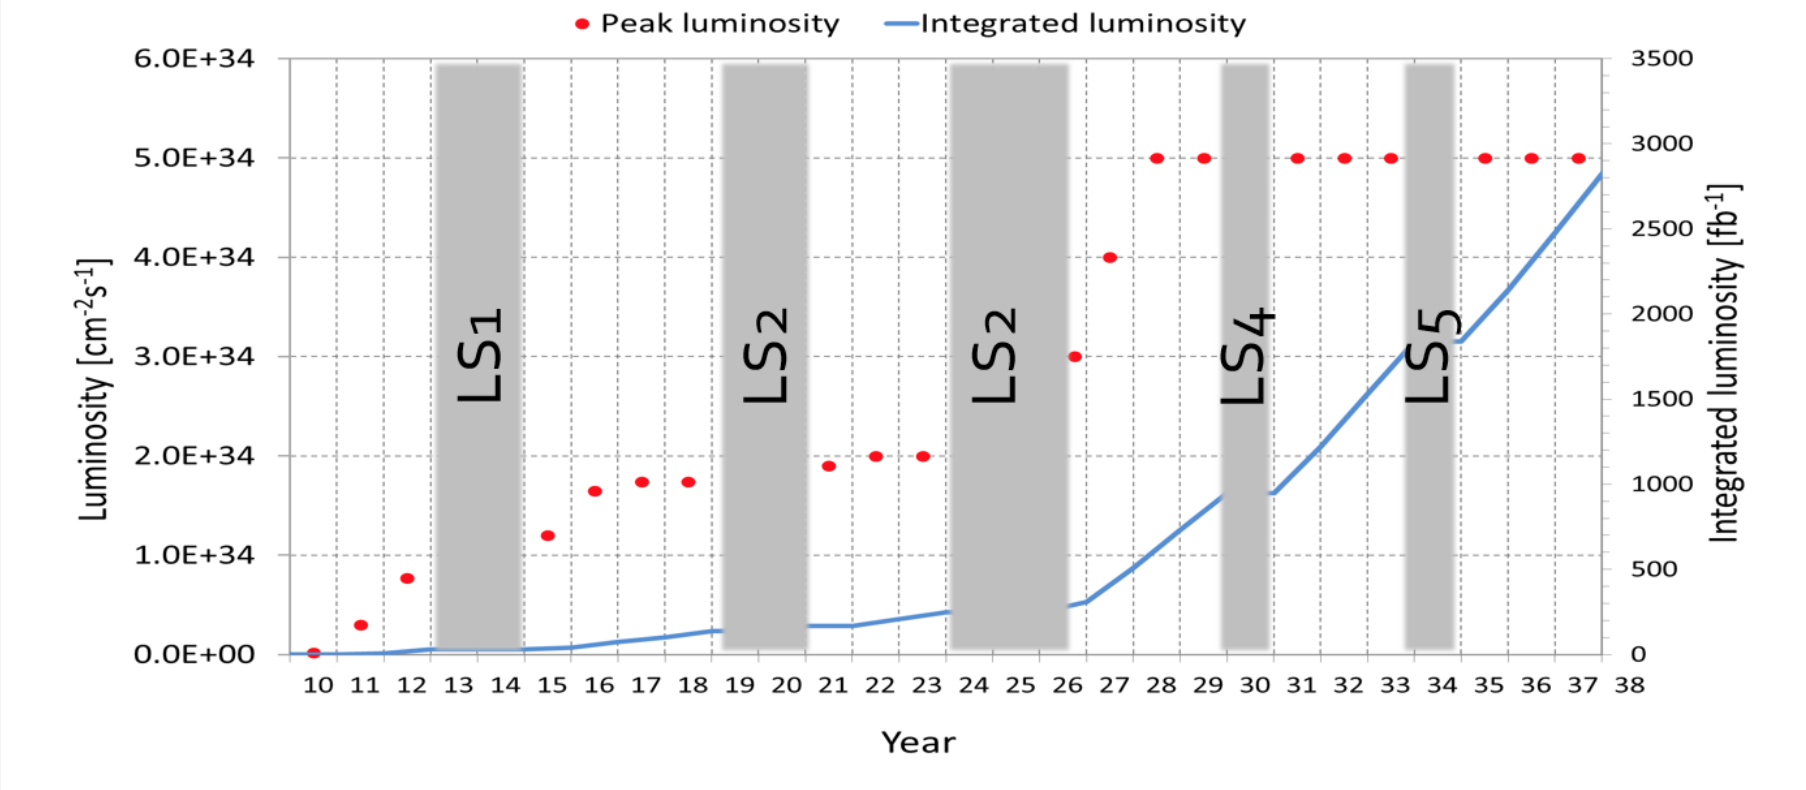
\includegraphics[width=0.95\textwidth]{CMS_experiment/LHC_integrated_lumi.png}
  \caption[Performance of LHC, extended to include the luminosity projections for up until the end of the HL-LHC phase.]{Performance of LHC, extended to include the luminosity projections for up until the end of the HL-LHC phase~\cite{ref:Schmidt_2016}}
  \label{fig:lhc}
\end{figure}


\hspace{10pt} Contents of the chapter following the completion of the LHC era are yet to be set in stone. A set of different proposals exist, with each of them having benefits and constrains in both monetary and physics sense of speaking. One highly advocated proposal is The Future Circular Collider (FCC) project~\cite{FCC_CDR}. It discusses a similar approach to one used with LEP/LHC years ago. During the early years of the project, an electron-positron collider would be built (FCC-ee) in order to probe the electroweak sector even further, while the technology is being prepared for the hadron collider (FCC-hh) that would bring the increase of the operational energy to the record level of 100~TeV. 



\subsection{The Compact Muon Solenoid}
\hspace{10pt} Taking the role of a leading general purpose detector\footnote{A completely unbiased observation by the author}, the CMS detector was designed to operate under proton-proton and ion collision beams with energies of 7 and 2.75~TeV respectively~\cite{cms:tdr}. It's design philosophy revolves around a few items, with the main, discovery of the Higgs boson, already  being marked as done early on during the initial Run 1 phase of LHC operation. As mentioned in the previous section, now the focus is to unravel what lies at the TeV energies, either through precision measurements and studies of known particles or by trying to search for new physics using theoretical models whose ideas can be quantified in a collider experiments. 



\section{Structure of the experiment}

\hspace{10pt}The CMS experiment itself is a cylindrical, layered detector comprised of several subsystems (as shown in Figure~\ref{fig:cms_slice}) working in harmony to help with particle detection and reconstruction. The subdetectors forming the CMS experiment are: the tracker, the electromagnetic calorimeter, the hadronic calorimeter, the superconducting solenoid, the muon chambers and the return yoke~\cite{cms:paper}. The general discussion of its operation can be split into two topics: the detection and data aquisition. Both of these will be covered in the following pages.
\subsection{Geometry}
\label{sec:geometry}
\hspace{10pt} The CMS experiment is positioned in a French village of Cessy, tucked in between beautiful sights of Jura mountains on one side and the city of Geneva from the other, allowing for a more descriptive approach when fixing the coordinate system~\cite{cms:tdr}. The main collision point is chosen to be the point of origin, from which the y axis follows the vertical line leaping towards the sky. The x axis is chosen as the one which points towards the center of the LHC ring, leaving the z axis to be the one that is tangent to the beam line, while also enjoying the view of the aforementioned mountains (as illustrated in Figure~\ref{fig:cms_coord_syst}).
\begin{figure}[htbp]
  \centering
    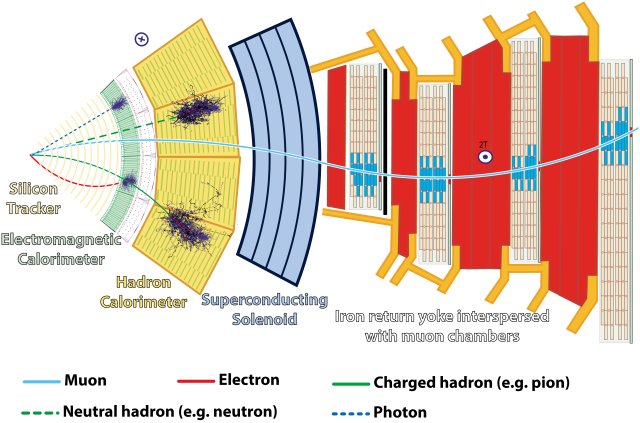
\includegraphics[width=0.85\textwidth]{CMS_experiment/CMSslice_whiteBackground.png}
  \caption[Transversal representation of different layers of the CMS experiment.]{Transversal representation of different layers of the CMS experiment~\cite{zCMS_slice}.}
  \label{fig:cms_slice}
\end{figure}
The definition of polar coordinates follows the standard procedure with the $\theta$ (polar) angle being defined from the z axis and the $\phi$ (azimuthal) angle being placed in the x-y plane starting from the x axis. In collider experiments it is usually easier do define alternative geometrical variables used to describe an object's position. This leads to the definition of peseudorapidity as: 
\begin{equation}
\eta = -ln\left [tan\left (\frac{\theta}{2}\right ) \right]
\end{equation}
Another variable commonly used to quantify the geometrical distancing of the particles is $\Delta R$. For two objects it is defined as:
\begin{equation}
\Delta R = \sqrt{\Delta\eta^2+\Delta\phi^2}
\end{equation}
Due to the structure of the CMS detector itself, it is important to define additional variables in the x-y, in further text the transversal (or the r-$\phi$), plane. Variables connected to it such as the transversal momentum and energy will be denoted as $p_T$ and $E_T$ respectively. The most important properties for this study are the missing transversal momentum and energy. They can be written as:
\begin{equation}
\begin{array}{l}
\vec{p}_{T, miss} = -\sum_i\vec{p}_{T,i},\\
E_{T, miss} = |\vec{p}_{T, miss} |,
\end{array}
\label{for:met}
\end{equation}
where the sum goes over all particles reconstructed by the detector. This imbalance in transversal momentum represents a valuable asset when quantifying the contribution of particles that are invisible to the detector. This will became more evident in the following chapters, where the $E_{T,miss}$ will be used extensively. 
Additional variables such as the transverse mass of a two body system, where particles masses can be neglected, can be written as:

\begin{equation}
    M_T = \sqrt{2E_{T,1}E_{T,2}(1-cos\Delta\phi)}.
\end{equation}

The following sections are going to further dissect the structure of the CMS experiment using the terminology introduced above. Two terms that will be a recurring item are the barrel and the endcap region representing a literal way of describing two general structural parts when discussing subdetector layers.
 
\begin{figure}[htbp]
  \centering
    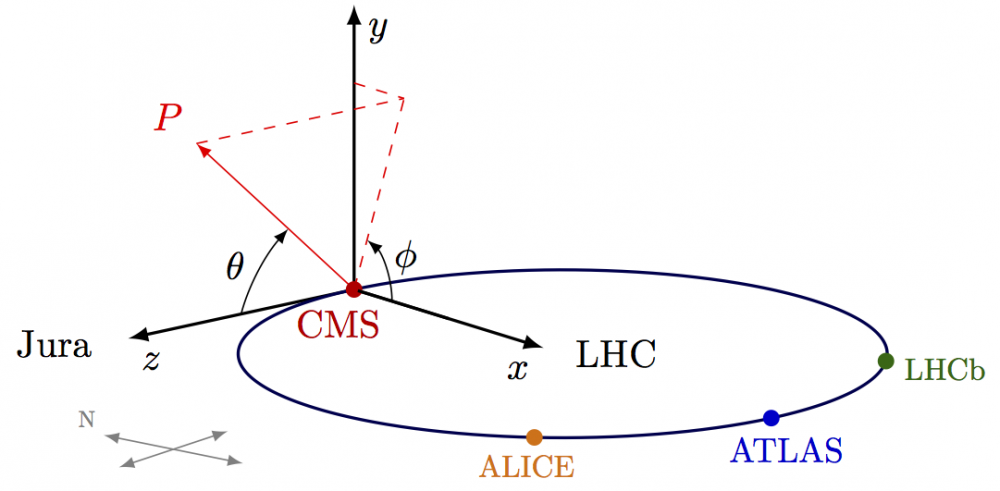
\includegraphics[width=0.8\textwidth]{CMS_experiment/cms_coordinate_system.png}
  \caption[Graphical representation of the coordinate system fixed to the CMS experiment.]{Graphical representation of the coordinate system fixed to the CMS experiment~\cite{coord_syst}}
  \label{fig:cms_coord_syst}
\end{figure}




\subsection{Tracker}
\hspace{10pt} The reconstruction of charged particle's track and the measurement of corresponding momenta is a crucial task for any collider experiment. The basis for tracking is formed around the interaction of charged particles with the atoms of the material they are travelling through. Said in a more precise way, the method revolves around exploring the trail of ionised atoms and free electrons left by particle moving in a magnetic field. If an electric filed is introduced in order to separate those electron-hole pairs, a current pulse will be created allowing for a "hit" signal to be detected.

\hspace{10pt} The, semiconductor based, tracking detector of the CMS experiment~\cite{cms:tdr}\cite{tracker_performance}\cite{Tracker:scheme} is positioned around the beam line, fully surrounding the interaction region as shown in Figure~\ref{fig:tracker}. It's design philosophy follows that it has to sustain the high collision rate given by the LHC, while providing the output in a form of particle tracks originating from the primary and secondary interaction vertices for the pseudorapidity range of $|\eta|<$2.5. The LHC input characteristics impose requirements that the tracker needs to have a high granularity structure, to provide longevity of the system and to have the ability to separate tracks originating from different bunch crossings (in other words, a fast enough response). All of this leads to the tracker being a fully silicon detector. The system itself is made out of two, operation independent, parts: the pixel detector (inner layer) and the the strip detector surrounding it bringing the total dimensions to 5.8~m in length with a 2.5~m in diameter (following the cylindrical design of the whole CMS experiment).
\hspace{10pt} 
\begin{figure}[htbp]
  \centering
    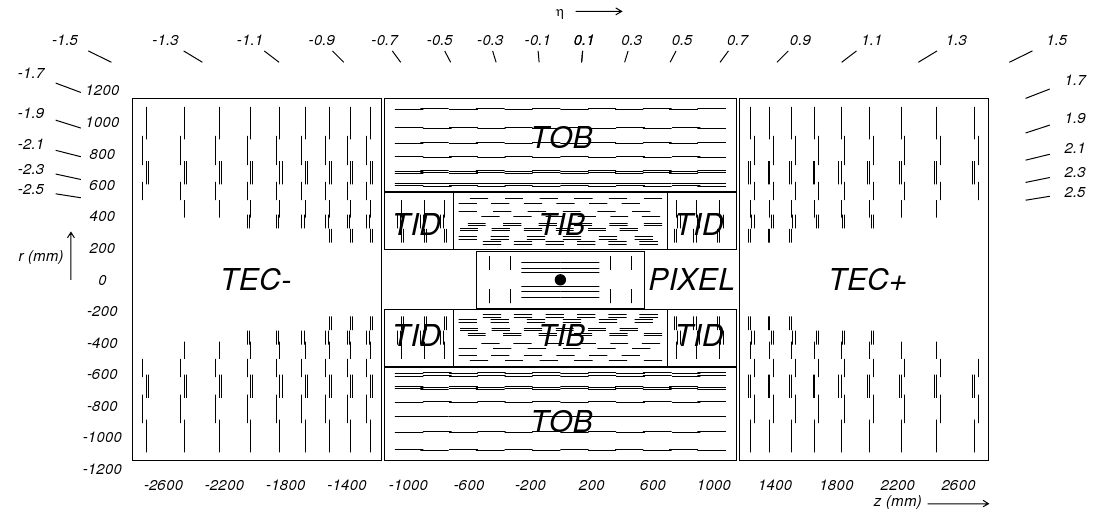
\includegraphics[width=\textwidth]{CMS_experiment/cmstracker.png}
  \caption[Structure of the CMS experiment's tracker system showcasing the subsystems in the barrel and endcap regions.]{Structure of the CMS experiment's tracker system showcasing the subsystems in the barrel and endcap regions~\cite{Tracker:scheme}.}
  \label{fig:tracker}
\end{figure}

\hspace{10pt} The pixel detector, covering the surface of 1.1~m$^{\text{2}}$, represents the first line of detection within the CMS experiment. Its barrel region (located within the $|\eta|<$0.9 range) is formed out of three cylindrical layers of detector modules with the radius being 4.4, 7.4 and 10.2~cm respectively. Forming the endcap region, additional two discs containing pixel modules are placed, completing the setup to a total of 66 milion pixels. It outputs three spacial points of detection associated to each charged particle in the event. The pixel subsystem represents an essential tool in reconstruction process of secondary vertices which play an important role in detecting heavy flavor and tau decay products. 

\hspace{10pt} The second part of the tracker, the strip detector, is made from a 10 layered barrel region and a set of 9 discs forming each endcap sides. The Inner barrel (TIB) and Discs (TID) form the first out of three main subsystems, delivering up to four detection points in the r-$\phi$ plane. The Tracker Outer Barrel (TOB) coveres the TIB and TID systems, allowing for additional points to be detected. Finally, shifting to the endcap region, there are the Tracker Endcaps (TEC+/-) providing up to nine $\phi$ detection points. Additional micro strip module is placed in all subsystems in order to enable the estimation of the missing component (r for the endcaps and z-axis position for the barrel).

\hspace{10pt} The importance of the tracking system is also seen in particle identification at the trigger decision level where the seed tracks are being constructed and passed as input data for the  trigger alogirthms to make an online decision.



\subsection{Electromagnetic Calorimeter}
\hspace{10pt} The next subsystem in particle's journey is the Electromagnetic Calorimeter (ECAL)~\cite{cms:paper}\cite{ECAL_performance}. It is comprised out of 75848 PbWO$_{\text{4}}$ (lead tungstate) crystals. The logic behind these types of detectors is based on the behaviour of high energy electrons and photons when passing through a material with a high atomic number Z. For the electrons, the main type of interaction with matter (in this energy range) is bremsstrahlung, while the photons interact through the electron-positron pair production. This, at the detector level, is cumulatively seen as an electromagnetic shower and is used to measure the energies of electrons and photons by amplifying the scintillation light produced in this process. Additionally to these e/$\gamma$ processes, there can be another contribution coming from $\pi^\text{0}$ decays to two photons originating from hardonic showers. The performance of the ECAL detector was crucial for the efforts towards the discovery of the Higgs boson. Its main driving force and ultimately its most important role was associated with searches within the $\text{H}\rightarrow \gamma\gamma$ decay mode (as well as the rest of modes containing $\text{e}/\gamma$ in its final state). 

\hspace{10pt} Scintilating crystals making the ECAL are chosen because of the compatibility of their properties with the expected performance of the LHC. The short radiation length (X$_\text{0}=\text{0.89}~\text{cm}$) ensures a small Moli\`ere radius (R$_\text{M}=\text{2.2~cm}$), allowing for compact dimensions of the detector. Being made out of a high density and optically clear crystal, ECAL can cope with the radiation impact as well as provide a compatibility with the bunch crossing time. The last statement translates into the fact that the majority of the scintillation light is being emitted in 25~ns. 

\hspace{10pt} The detector is made out of a barrel section which is hermetically sealed with the encap sections. The ECAL barrel (EB) section is responsible for energy deposits left within the $|\eta|<$1.47 range while the Endacap (EE) sections take over the responsibilities for the 1.68$<|\eta|<$3.0 range. The EB/EE crystals are $\approx$25/26 X$_\text{0}$ in length respectively. This choice of dimensions for the side facing the particle's trajectory is motivated by the size of the EM shower left in the crystal. Having such frontward crystal dimension simplifies the particle identification as the shape of the shower can easily be added as a selection criteria. A more visual overview is given in Figure~\ref{fig:ecal}, which showcases the structure of the ECAL where the aforementioned crystals are arranged in 36 supermodules. In order to have another helping hand, a preshower detector, which acts especially when it comes to $\pi^\text{0}/\gamma$ separation, is added to the setup. It is positioned in front of the EE rings covering the 1.64$<|\eta|<$2.5 region with its set of lead absorbers and silicon strip sensors.
\begin{figure}[htbp]
  \centering
    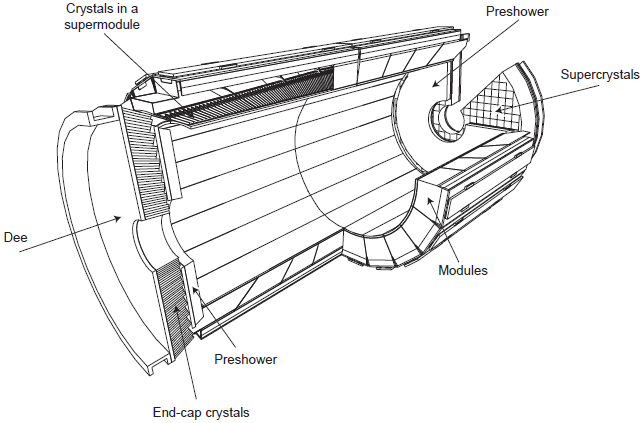
\includegraphics[width=0.8\textwidth]{CMS_experiment/CMS_ECAL.png}
  \caption[Schematic view of the CMS ECAL subdetector. The main susystems (EB, EE and the preshower detector) are presented as well their substructure]{Schematic view of the CMS ECAL subdetector. The main susystems (EB, EE and the preshower detector) are presented as well their substructure~\cite{cms:ecal}.}
  \label{fig:ecal}
\end{figure}

\hspace{10pt} With all the benefits that this choice of crystal structure brings, there are bound to be certain downsides. One additional property of lead tungstate cristals is that they have a very low light yield.  A set of signal amplifiers is needed in order to battle this disadvantage. For the EB region, a set of silicon avalanche photodiodes (APD) is used to boost the signal by a factor of $\sim$50 compared to the original. A similar scenario is deployed for the EE region, where vacuum phototriodes (VPT) with amplification ability of $\sim$10 times are used.

\hspace{10pt} The energy resolution of the ECAL detector can be parametrised as:
\begin{equation}
    \frac{\sigma^2}{E^2} =\bigg (\frac{A}{\sqrt{E}}\bigg )^2 +\bigg (\frac{B}{E} \bigg )^2 + C,
\end{equation}
where A, B and C represent the stochastic, noise and constant term respectively. The stochastic term is measured to be $2.8~$\% . The noise term, comprised form the cumulative effects of pileup, electronics and digitasion noise, has the value of $12~$\%. Finally, the constant term of $0.3~$\% is assigned to account for any leakage of energy or inter calibration errors. 

\hspace{10pt} The story of the ECAL will continue in Section~\ref{sec:data_acquisition}, where it will be showcased how these outputs are used at the first level of selection and beyond.
\subsection{Hadronic Calorimeter}
\hspace{10pt} Following a similar path derived for detecting the residuum of electromagnetic interactions of particles, a separate detector system has been added to measure the energies of hadronic showers - the Hadronic Calorimeter (HCAL)~\cite{cms:paper}\cite{hcal_performance}. When neutral and charged hadrons interact with the detector material through strong interaction, a hadronic shower will be formed with associated parameter $\lambda_{\text{i}}$, the nuclear interaction length. Representing a mean distance beween hadronic interactions within the shower, it takes much larger values than its electromagnetic equivalent, the radiation length. This would imply that the HCAL has to have large dimensions in order to be efficient, but on the other hand the compactness of the CMS detector fixes its position (and maximum dimensions) right in between the ECAL and the solenoid coil. This potential disadvantage is overcome with the structural design of the HCAL, which is made out of: barrel/endcap sections (HB/HE), a Hadron Forward (HF) subdetector and the outer barrel hadronic calorimeter (HO). Figure~\ref{fig:hcal} showcases the structure of the HCAL and all of its aforementioned parts.


\begin{figure}[htbp]
  \centering
    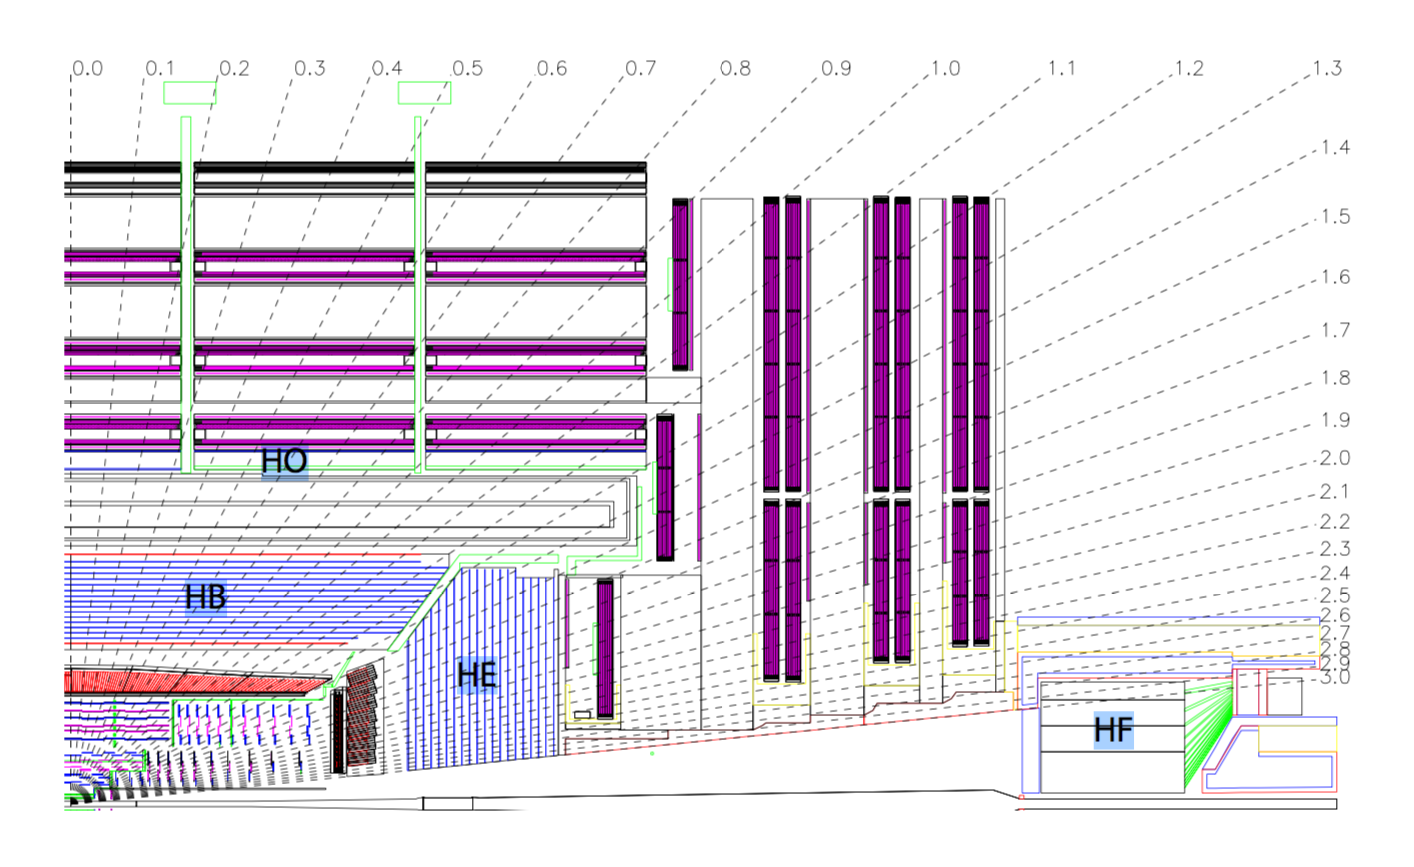
\includegraphics[width=0.95\textwidth]{CMS_experiment/HCAL_structure.png}
  \caption[Schematic ($\text{r}-\text{z}$) view of the CMS HCAL detector highlighting different subsystems: the hadronic barrel/endap (HB/HE), forward (HF) and outer (HO) detectors.]{Schematic ($\text{r}-\text{z}$) view of the CMS HCAL detector highlighting different subsystems: the hadronic barrel/endap (HB/HE), forward (HF) and outer (HO) detectors~\cite{cms:paper}}
  \label{fig:hcal}
\end{figure}

\hspace{10pt} The HCAL barrel is itself comprised out of two identical halves (HB$^{\text{+}}$/HB$^{\text{-}}$) covering the $|\eta|<$1.3 region. The subsystem is made out of layers of brass/steel (absorbing material) and scintillator tiles. A total of 32 identical wedges (each being segmented into four $\phi$ regions) made out of absorber plates form each of the barrel regions, with the scintillator tiles being positioned into 16 $\eta$ regions, bringing the total segmentation to ($\eta$, $\phi$) = (0.087, 0.087). The absorber itself is formed out of a front and back set of steel plates, in between which resides a group of 11 thick brass plates. The total thickness varies with $|\eta|$ from 5.8 until 10.6~$\lambda_{\text{i}}$ (for the edge values of $|\eta|=$0 and 1.3 respectively). On top of the HB thickness, there is a contribution coming from the previous detector, where the ECAL brings an additional 1.1~$\lambda_{\text{i}}$ to the total value. The scintialltor tiles are equipped with wavelength shifting fiber (WLS) readout, which is responsible for the transfer of emitted optical light. In order to battle the, previously mentioned, constrain in barrel dimensions, another subsystem is added after the solenoid structure (covering the $|\eta|<$1.26 region). The addition of the outer barrel hadronic calorimeter (HO) serves to effectively extend the size of the barrel section by moving the minimal thickness value up to 11$~\lambda_{\text{i}}$.

\hspace{10pt} Moving on to the endcap secion (HE), a set of two subsystems are put in place to be in charge of the 1.35$<|\eta|<$3.0 region following the same brass/scintillator structure used in the HB sections. Covering the diameter region starting from 0.8~m until 6.0~m, the endcaps have the same ($\eta$, $\phi$) segmentation as the HB sections for almost the entire $\eta$ range (the edge case being the $|\eta|\sim$3.0 region, where it doubles in value). A set of two forward calorimeters (HF) is placed behind the ends of the HE section. Each of them represents a Cherenkov detector comprised out of quartz fibers placed into iron and are used due to their radiation durable properties to extend the coverage up to $|\eta|<$5.2 (placing it really close to the beam line).


\subsection{Magnet}
\hspace{10pt} The central component of the CMS experiment (and one third of its name) is the 4~T superconductive solenoid~\cite{cms:paper} used to curve the trajectories of charged particles. It is 12.5~m long cylindrical structure with a diameter of 6~m. A high number of ampere-turns needed in order to generate such a strong field (41.7 MA-turns), introduced a new, four layer winding design which was a clear departure from solutions used with previous experiments (maximum of two layers). During run periods, the value it operates on is bellow its design value and stands at 3.8~T in order to ensure the durability of the system as a whole.

\hspace{10pt} Another important part of the magnet system is the return yoke. It is made out of 5 wheels in the barrel and 3 discs per endcap section interspersed alternately between layers of Muon chambers (described in the following section). Contibuting to the majority of the CMS experiments' weight, it stops almost all particles reaching it (minus the muons and neutrinos).
\subsection{Muon Chambers}
\label{subsec:cmsmuon}
\hspace{10pt} The final detector system discussed in this chapter are the muon chambers. Being a focal point for one of the main searches for the SM Higgs boson, the four muon final state represents the cleanest signature out of all other four lepton combinations due to the fact that muons are the least affected by energy loss in the previous sections (namely the tracker). This has influenced the way the CMS experiment was designed in a similar way how ECAL was connected to the diphoton final state. In order to approach the detection of muons, a setup is created through the use of three subsystems~\cite{cms:paper}\cite{muon_chambers_proceedings} based around gas chambers. 

\begin{figure}[htbp]
  \centering
    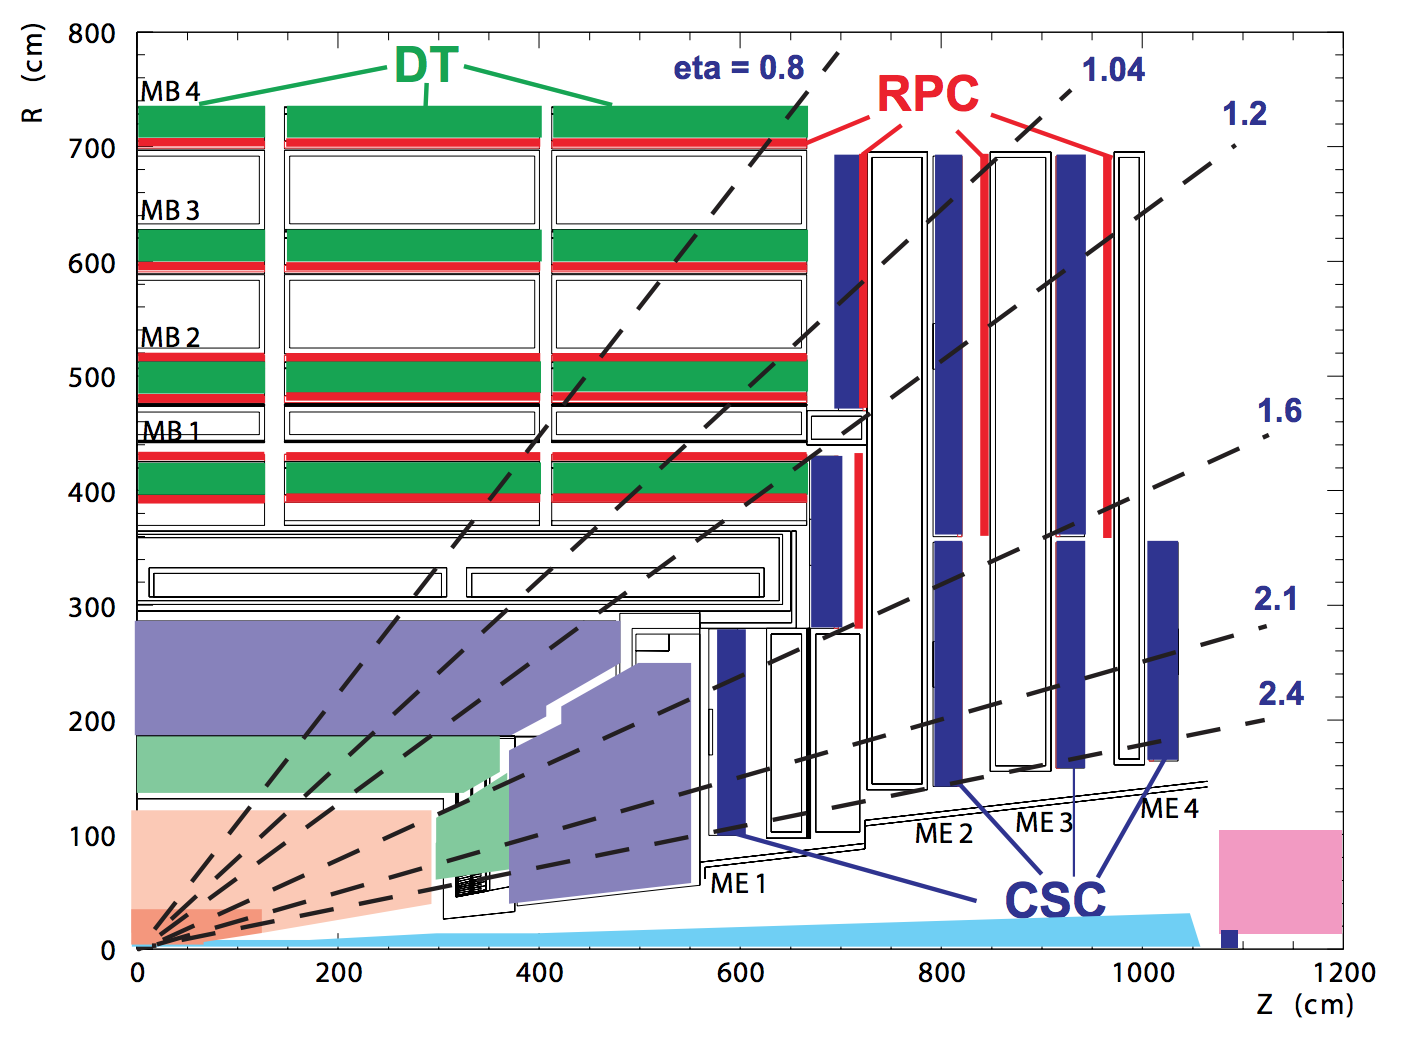
\includegraphics[width=0.95\textwidth]{CMS_experiment/Muon_chambers.png}
  \caption[Structural design of a ($\text{r}-\text{z}$) slice of the CMS Muon system highlighting different subsystems: the DT, CSC and RPC detectors.]{Structural design of a ($\text{r}-\text{z}$) view of the CMS Muon system highlighting different sections: the DT, CSC and RPC detectors~\cite{cms:tdr}}
  \label{fig:muon_chambers}
\end{figure}

\hspace{10pt} Starting from the barrel section, the $|\eta|<$~1.2 region is covered through the usage of Drift Tube (DT) chambers. From the stuctural point of view, each DT is made out of a streched wire placed in a gas volume. Comprised out of four stations inserted within the yoke, DT subsystem is responsible for measurement of muon's coordinates for this $\eta$ range. The first three inner stations (each containing 60 chambers) are responsible for mapping in both the r-$\phi$ plane as well as the z axis projection, while the last station (comprised out of 70 chambers) lacks the latter ability. For the encap region, a set of Cathode Strip chambers (CSC) is used instad of DTs. The change in the approach was introduced due to a much larger muon rate in this region, where radiation harder material and faster response given by the CSCs has proven to be a better option. 

\hspace{10pt} In order to battle the large amount of information, a dedicated trigger has been introduced to both DTs and CSCs. Based on the Resistive Plate chambers (RPC), this system is expected to provide fast triggering response over the majority of the $\eta$ range ($|\eta|<$1.6), helping out with muon track reconstruction scenarios starting from multiple hits per chamber (in case of DTs and CSCs). They employ the double gap chamber structure which in return provides good performance during full operation. The barrel section contains six layers of RPCs, while the endcap has areas covered with them for the first three sections, positioned in such way to complete the setup for an efficient (compact) muon detection system. 








\chapter{Data Acquisition}
\label{ch:daq}
%\label{sec:data_acquisition}
%\normallinespacing
\setlength\epigraphwidth{.8\textwidth}
\setlength\epigraphrule{0pt}
\epigraph{\itshape``It has long been an axiom of mine that the little things are infinitely the most important."}{--- \textup{Sir Arthur Conan Doyle, The Memoirs of Sherlock Holmes}}
%\mediumlinespacing
\section{Introduction}
\hspace{10pt} The sheer amount of data brought by the LHC brings a lot of opportunities for physicists to explore at the TeV scale. As it is usually the case, one advantage also brings a plethora of difficulties that need to be overcome, usually requiring a more practical approach. When looked at the maximum collision rate at the LHC (40~MHz), it can be seen that the total stress on the data acquisition system is around 40 million collision events per second, which is far beyond the reach of any currently available data storage systems. In order for the CMS experiment to be able to perform as efficiently as planned, a two stage structure was deployed with a task of discarding events deemed "unworthy" by its logic.

\hspace{10pt} Facing this problem head on, the CMS triggering setup consists of a, hardware based, first level of selection - the Level-1 Trigger (L1T) and a software High Level Trigger (HLT). The initial selection process done using the L1T scales down the total input rate to, a more approachable, 100~kHz. These decisions are based around a limited set of information coming from a set of subdetectors. The next stage in the triggering process, the HLT selection, is designed to further reduce the resulting output to $\sim$1~kHz of data, which is manageable by both the storage and offline reconstruction systems. Each of these triggering levels has a dedicated set of algorithms combined into a structure called the trigger menu. It is designed with the goal of allowing the passage of the appropriate rate of events expected from that system. The following sections are going to showcase the structure for each of these triggering levels, while focusing on examples relevant to the main study presented by this thesis.

 \section{Level-1 Trigger}
 \hspace{10pt} The starting point of this discussion is the, as the name suggest, first level of selection within the CMS experiment~\cite{cms:l1_paper}. It stands at the front line of data acquisition and is tasked with making a fast (in less than 4~$\mu$s) but sensible decision whether an event should be passed further down the chain. The core of the entire setup are the Field Programmable Gate Array (FPGA) boards. Their ability to perform faster parallel processing, re-programmability and the subsequent good price to performance/durability ratio, have lead to them being chosen instead of a CPU architecture. The many advantages that come with using the FPGAs in highly specialized tasks have lead to their wide spread usage, reaching even the video game industry\footnote{FPGAs are being used in modern recreations of 16-bit custom chips making the core of the fourth video game console generation such as the ones found in the Super Nintendo Entertainment System and Sega Mega Drive systems.}. The following pages are going to focus on the structure of the Level-1 trigger, relaying on a set of examples to efficiently explain its operation.
 
 \subsection{Overview}
 \label{l1:TTs}
 \hspace{10pt} The L1T forms a decision relying on the information coming form two centres: Calorimeters and Muon chambers. This can be seen in Figure~\ref{fig:l1_structure}, which shows the structure of the L1T system during the Run 2 phase of operation. Named after the corresponding information pool, the substructure of the L1T can be split into the Calorimeter and Muon trigger. The Calorimeter (Calo) trigger is comprised out of two layers and is responsible for the reconstruction, calibration and baseline identification of particles with ECAL/HCAL deposits: electrons/photons (e/$\gamma$), tau ($\tau$) and hadronic jets. The aforementioned jets represent a residuum of hadronic interaction located within a narrow geometrical cone. Due to the lack of tracker information at this stage, it is not possible to distinguish electrons from photons, which is why they are referred to as e/$\gamma$ objects. On the other hand, the Global Muon Trigger (GMT) is used to summarise the information gained from the three muon subsystems previously defined in Section~\ref{subsec:cmsmuon}. The starting point for both of these triggers is the same and comes from the information provided by the trigger primitives (TPs) which are formed from basic detector units.
\begin{figure}[htbp]
  \centering
    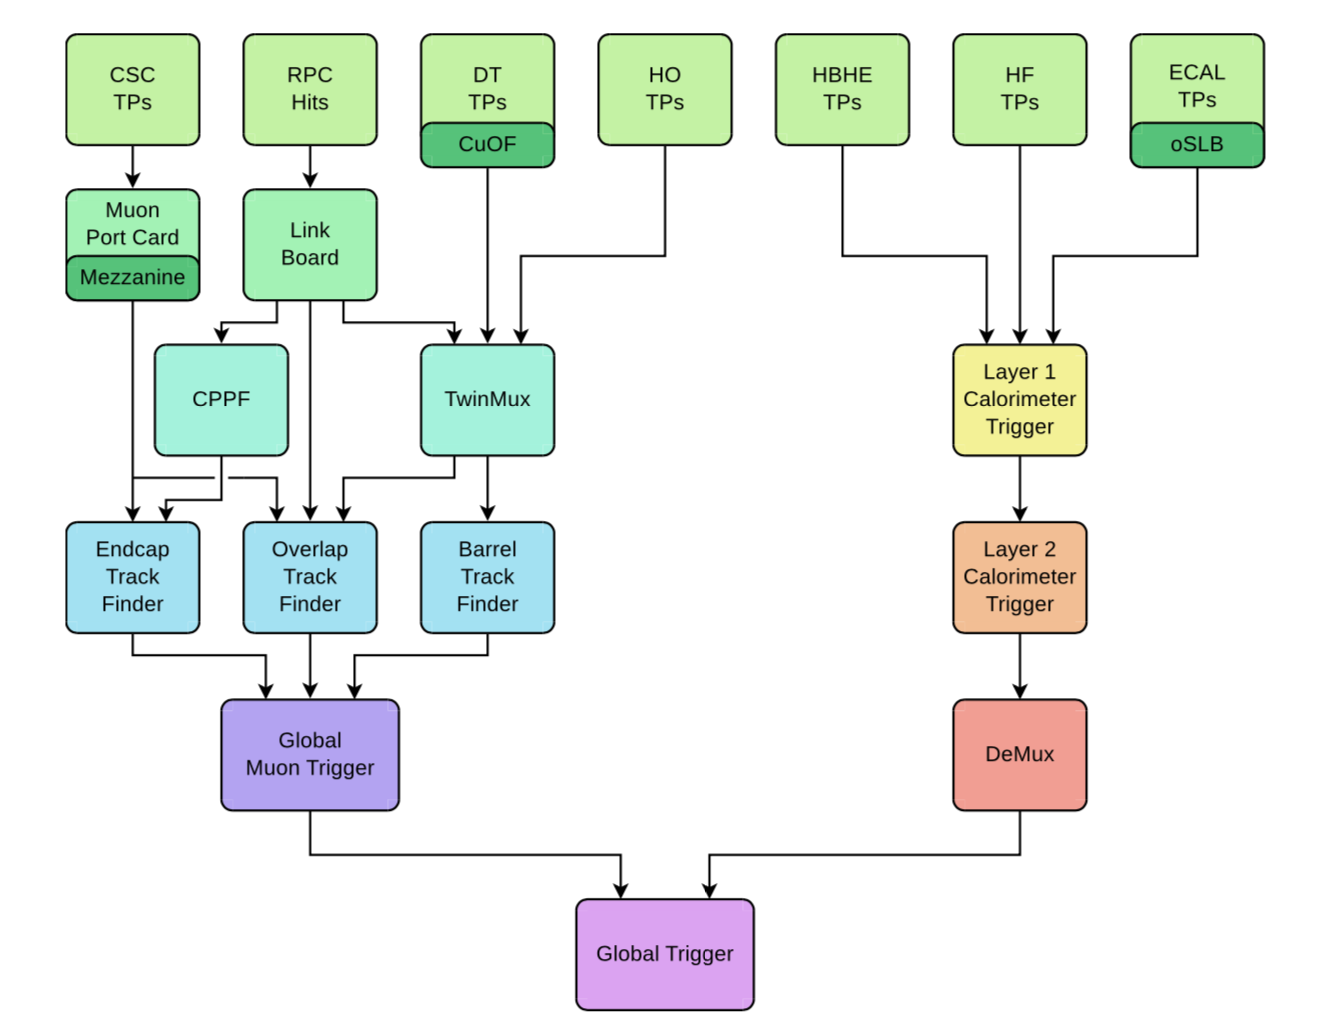
\includegraphics[width=0.95\textwidth]{CMS_experiment/L1_diagram.png}
  \caption{Structure of the CMS Level-1 system during its Run 2 operational phase.~\cite{cms:l1_paper}}
  \label{fig:l1_structure}
\end{figure}

\hspace{10pt} Figure~\ref{fig:l1_calo_trig} shows the structure of the Calo trigger. Detector inputs for this system are made out of Calo Trigger Towers (TTs). Each of these TT represents a 5x5 ECAL crystal structure combined with the HCAL tower positioned behind it [R] formed as such to take the advantage of the full detector granularity . The information (energy deposits) coming from TTs is passed to the Calo Layer-1. These deposits are then calibrated, corrected for additional detector effects (not accounted by the calorimeter electronics) and sorted preparing the input for the next step.

\hspace{10pt} The Calo Layer-2 is comprised out of a set of 9 FPGA cards (MP7), connected together in a round robin scheduling sequence. This Time-Multiplexed Trigger (TMT) design helps to extend the processing time given to each of the Calo Layer-2 cards. As an example, if each of the boards received information regarding one event per bunch crossing using this TMT design, this would increase the available processing time to be nine times larger than the standard bunch crossing time. At this stage, Calo L1 objects are being reconstructed from the available information using dedicated algorithms. The resulting data stream is being passed onto the De-multiplexing node (Demux), another MP7 board, with the task of retrieving the original event ordering before sending this information to the Global Trigger ($\mu$GT).
\begin{figure}[htbp]
  \centering
    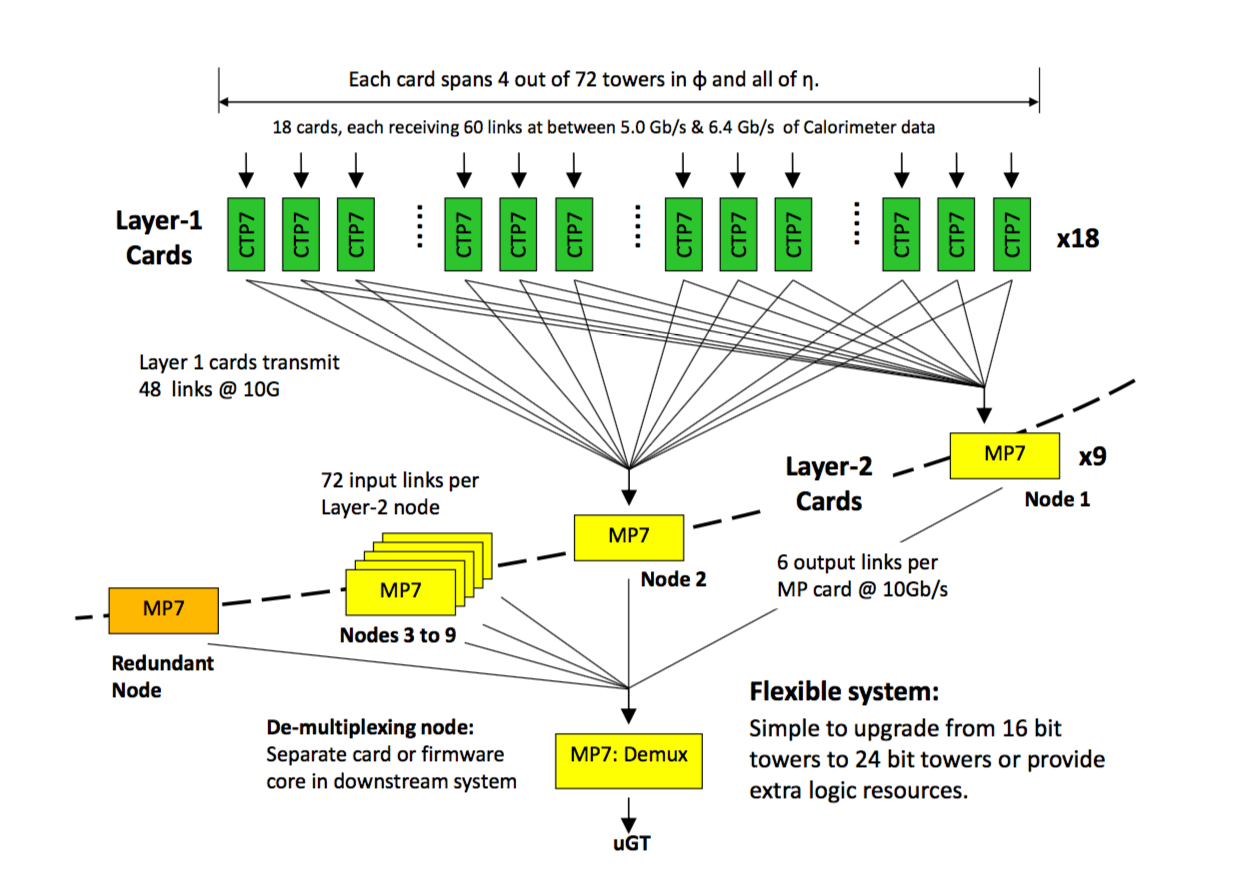
\includegraphics[width=\textwidth]{CMS_experiment/L1_calo_trig.png}
  \caption{Structure of the Calorimeter Trigger and its Time-Multiplexed Trigger architecture.~\cite{cms:l1_paper}}
  \label{fig:l1_calo_trig}
\end{figure}

\hspace{10pt} Due to their connection with the VBF production mode and the subsequent invisible final state of the Higgs boson, jets and energy sums will be used to illustrate L1T reconstruction algorithms~\cite{cms:l1_paper}\cite{Antoni}. Reconstruction of jets at L1T is performed through the usage of a dedicated algorithm. It focuses on a 9$\times$9 TT range surrounding the TT with the maximal deposit within the area, which satisfies the $E_T>$~4~GeV requirement. This TT range is chosen to mimic the geometrical ($\eta$, $\phi$) area used with offline jet reconstruction, which revolves around the $\Delta$R~$<$~0.4 cone. A simple comparison of energies with the TTs surrounding the central one are performed and the central TT is selected as a jet "seed" candidate if no other TT in the 9x9 area has energy larger/larger or equal than it. This additional equality comparison has been added in order to remove the possibility of the effect when TTs with same energies mutually veto each other. The chosen convention is shown in Figure~\ref{fig:l1_jet_chunky}. The total energy associated with the jet is then computed by summing the contribution from all TTs in the area, while the jet position is being fixed to the central seed TT. 

\hspace{10pt} Subtraction of the pile-up\footnote{Additional interactions whose resulting signatures are overlapping with the interaction of interest. It is coming from the fact that the LHC collides bunches of protons instead of a single pair.} contribution is done by using a set of four 3x9 TT structures, positioned next to the edges of the original 9x9 structure. This combined set of TTs bears a similarity with a "chunky doughnut", which is the initial idea behind the name of this jet pile-up removal algorithm. In order to avoid the scenario where a contribution coming from another jet structure would be removed, pile-up $E_T$ is computed using the sum of the three regions with the lowest energy which is then subtracted from the jet candidate energy.
 
\begin{figure}[htbp]
  \centering
    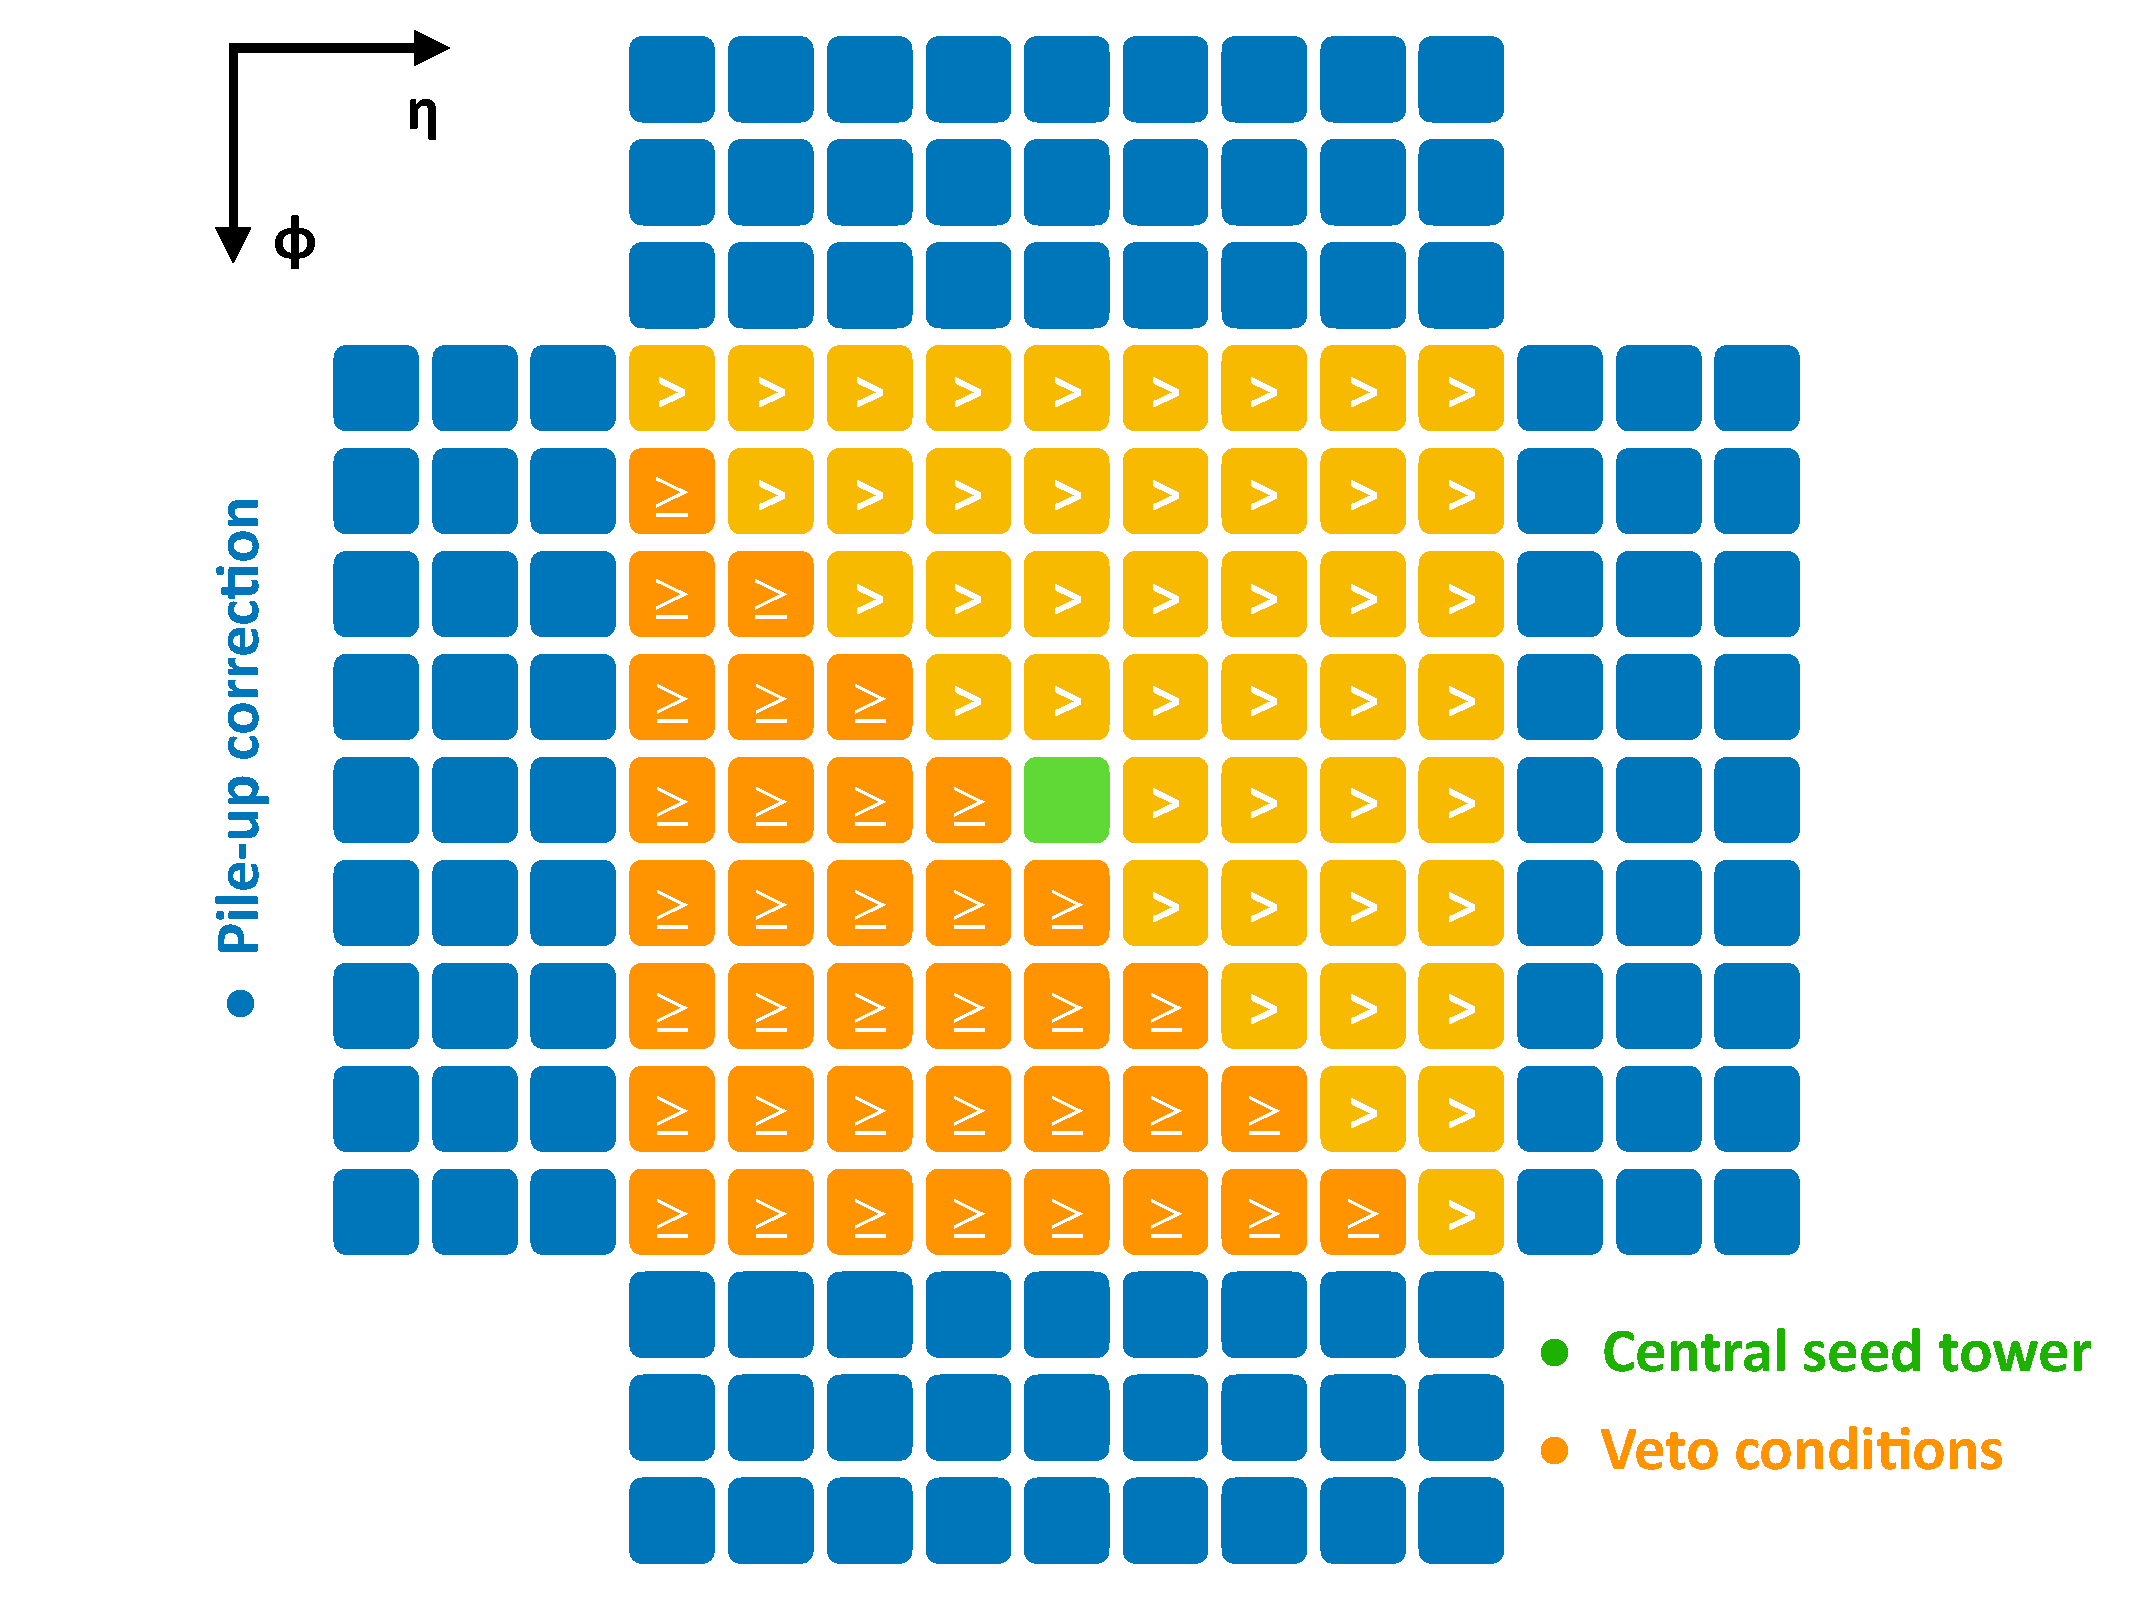
\includegraphics[width=0.9\textwidth]{CMS_experiment/jet_chunky.pdf}
  \caption{Graphical representation of 9x9 Calo TT formation used for L1T jet reconstruction, accompanied by 3x9 structures used for the pileup removal.}
  \label{fig:l1_jet_chunky}
\end{figure} 

Using the energies of the TTs it is possible to reconstruct the $\vec{p}_{T,miss}$ vector following the formula:
\begin{equation}
 \vec{p}_{T,miss} = -\sum_{i=1}^{n_{\eta}}\sum_{j=1}^{n_{\phi}}(E^{i}_{T}cos(\phi_j)\vec{e}_x + E^{i}_{T}sin(\phi_j)\vec{e}_y)
\end{equation}
 where (i, j) denote the sums over the ($\eta$, $\phi$) coordinates of TTs. Upon obtaining this property, the L1T $E_{T, miss}$ variable, extensively used when creating trigger paths listed in Table~{R} can be constructed as $E_{T, miss} = |\vec{p}_{T,miss}|$. Additionally, if the summation, when forming the previously defined property, goes over jet objects instead of all TTs, a new variable $\vec{H}_{T,miss}$ is created. 
 
\hspace{10pt} These physics objects reconstructed by the Calo Layer-2 are being passed on to the final step, the $\mu$GT, where they are combined with the information coming from the Muon trigger. At this stage, a decision is being made whether the event is going to be passed on to the HLT or discarded. In order to be able to make a decision, L1T uses a set of algorithms (seeds) which impose selection requirements on available physics objects. If the event passes all the requested qualities/thresholds and if the event is in accordance with the trigger rules, a Level-1 Accept (L1A) decision is being made and the event is passed on to the next step.

\subsection{Level-1 Trigger Menu}

\hspace{10pt} A set of aforementioned decision making algorithms, combined together through a logical "or", creates a structure called the L1T menu. The total rate of events selected by the menu is expected to be no larger than 100~kHz. In order to measure the collective rate given by the menu, an unbiased dataset (ZeroBias) is needed. The name ZeroBias is reflective of the fact that this data was collected using a selection that imposes only a single requirement: the event needs to contain a collision. 

\hspace{10pt}In order to control the total rate of events at the L1T, each seed within the menu has a "prescale" option inserted in the workflow. It provides the ability to limit the number of events passing the algorithm by scaling it down using a given integer value. This results in a scenario where, for a prescale value of 10, every tenth event which satisfies conditions imposed by the seed, is being allowed to advance to the next stage. 

\hspace{10pt} The implementation process for a new seed follows a standardised flow. Whether it being a simple or a complex algorithm, it's efficiency needs to be measured using Monte Carlo (MC) simulation samples that have been produced with appropriate object reconstruction. The increase in rate of the trigger menu associated with the addition of a new seed is called its pure rate. It has to be low enough for the trigger to be added to the menu, without removing/prescaling other seeds. The majority of the trigger menu rate is dedicated to seeds that have a wide spread usage in the later stages. Good examples of this are Single/Double lepton and $E_{T,miss}$ triggers, whose logic is presented in Table~\ref{tab:l1_triggers}. 

\begin{table}[htbp]
    \centering
    \begin{tabular}{lc}
     Algorithm & Requirements \\   \hline\hline
           & \\
      Single Muon   &  Tight Qualty \& $p_T>$22~GeV \\
                 & \\
      Double Muon  &  Tight Quality \& $p_T>$8~GeV  \\
                 & \\
      Energy sums ($E_{T}^{miss}$) & $E_{T}>$100~GeV \\
      & \\\hline\hline
    \end{tabular}
    \caption{A selected set of examples of most-used unprescaled trigger algorithms with their corresponding logics~\cite{cms:l1_paper}.}
    \label{tab:l1_triggers}
\end{table}

\hspace{10pt}For example, the lowest threshold, unprescaled single muon trigger is looking for a tight quality muon object that has $p_T>$~22~GeV. Muon objects that have been registered in at least three muon stations are marked down as tight quality objects. It is also possible to design triggers that would handle complex object manipulation. One of new seeds taking this advantage is created for the purposes of selecting VBF events. More details about this seed are going to be presented in Section~\ref{l1:vbf}. Finally, in order to safeguard the menu from any unforeseen rate problems, it is a common practise to have a few backup options for each seed. They are implemented with the same logic as the original, but with slightly higher thresholds on selection requirements. They provide viable replacements in situations when the menu rate is too high and the primary seed needs to be prescaled until the issue is fixed. 

\subsection{Level-1 Trigger pre-firing}
\label{sec:l1_prefire}
\hspace{10pt} Due to the heavy conditions under which the ECAL is exposed during LHC operation, a loss in transparency in its crystals began to affect its performance during 2016. With time this effect gradually increased, with the high $|\eta|$ regions being the most affected. This has introduced a timing offset in calibration of ECAL pulses, an effect that translated into resulting detector information which was turned into subsequent L1T Calo TPs. As a consequence of this, the Calo trigger information for the $|\eta|>$2.5 could be wrongly assigned to the previous (BX~$=$~-1) bunch crossing instead of the correct one (BX~$=$~0). This can lead to two major effects regarding the L1T decision.

\hspace{10pt} Firstly, it can lead to the effect called the L1T pre-fire in which the system wrongly distributes the information that the BX~$=$~-1 event passes its logic to the HLT. As this effect is not present with the offline reconstruction, a simplified version of which the HLT uses when reconstructing objects, pre-firing will cause the total loss of an interesting event. This comes from the fact that BX~$=$~-1 event will most likely be rejected at the HLT level due to the low probability that both BX~$=$~0 and -1  will contain interesting physics processes. On the other hand, accounting for the part of trigger rules which state that no more than one L1A decision can be made for three successive events (and no more than 2 L1As in a group of 25 successive events), the BX~$=$~0 event in this case is lost.

\hspace{10pt} Another scenario can happen due to a possibility of biased measurement of energy deposited in the Calo TPs. If the situation is reversed and the "early" signal does not invoke a positive L1A decision, there is still a problem as the, potentially interesting, BX~$=$~-1 information will be wrongly lost causing a bias in the energy measurement for the BX~$=$~0 event. 

\hspace{10pt} Unfortunately, a good example of a study affected by this issue is the VBF H$\rightarrow$inv analysis, due to its dependence of forward jets~\footnote{Jets within the forward region ($|\eta_j|>$~2.4)}. The effect of this has been studied at the analysis level for the data collected in 2016 [R] and the results state that a correction ranging from 1-20~\% needed to be applied (depending on the fit variable range), which resulted in a total loss of $\sim$17~\% of the expected sensitivity towards the BR(H$\rightarrow$inv). More details about the corrections of this issue for the data collection era of 2017 are given in Section~\ref{sec:objects}.


\section{Online Data Quality Monitoring}
\hspace{10pt} In order to have constant surveillance of the operation of the CMS experiment, three daily shift crews are placed at the control cavern at of the detector (positioned at the LHC Point 5). The constant monitoring of L1T menu rates is needed to quickly account for any unexpected increases, by prescaling problematic seeds. On the other hand, in order for the shifter to be able to monitor the performance of the L1T, as set of  informational plots and alarms is displayed as a part of the data quality monitoring (DQM) package~\cite{Antoni}. Taking into account that the knowledge possessed by the shifter is usually not on the level of a L1T expert, a separation of plots is being made into two groups: shifter and expert, where the latter contains much more details (i.e. the full Calo granularity information) needed for debugging.

\hspace{10pt} Taking the Calo trigger as the example, in order to have a separate control system, an emulator software was written in C++ and optimised for a CPU architecture with the same logic as the one used on the trigger boards (both the MP and Demux nodes). This emulator was made a part of a standardised CMS Software Framework (CMSSW), which helps with the general ease of use and software compatibility. In order to monitor the performance of the Calo trigger during run periods an online DQM package was deployed containing several main checks needed for validation.

\hspace{10pt} There are several types of plots needed to efficiently control the operation of the Calo Layer-2 during data taking periods. One of the first checks would be to plot the distributions of main properties of physics objects in order to quickly spot any anomalies in the reconstruction. On the other hand, the "data to emulator" plots sorted either by the overall agreement or disagreement between the firmware and the emulator represent a systematic way of ensuring early problem detection.  A select set of example plots summarising this setup are given in Figure~\ref{fig:dqm_plots} 
\begin{figure}[htbp]
  \centering
      \subfigure[A]{
    \includegraphics[width=0.45\textwidth]{example-image-a}
    }
    \subfigure[A]{
    \includegraphics[width=0.45\textwidth]{example-image-a}
    }\\
    \subfigure[B]{
    \includegraphics[width=0.45\textwidth]{example-image-a}
    }
    \subfigure[B]{
    \includegraphics[width=0.45\textwidth]{example-image-a}
    }\\
    \subfigure[C]{
    \includegraphics[width=0.45\textwidth]{example-image-a}
    }
    \subfigure[C]{
    \includegraphics[width=0.45\textwidth]{example-image-a}
    }
  \caption{DQM Example plots - TBA as soon as I get the online playback running.}
  \label{fig:dqm_plots}
\end{figure}


\section{High Level Trigger}

\hspace{10pt} The second step of trigger selection operates under more manageable input conditions, allowing for a few hundred millisecond decision making time window. This has enabled the more traditional, high level software, design of the High Level Trigger (HLT)~\cite{HLT_performance}. It is based on a set of algorithms (paths) written in C++, that are deployed on a server farm comprised out of Intel Xeon CPU based machines.

\hspace{10pt} This additional timing allows for more complex object reconstruction, which is why the HLT uses a simplified version of the Particle Flow (PF) algorithm in order to take the advantage of the full detector information. More details about the PF algorithm itself will be given in Section~\ref{sec:objects}. The main feature of the HLT is its modular design. A collection of C++ modules allows experts to build more detailed selection requirements. A module can take a role of a producer of $E_{T,miss}$ variable from given PF candidates, it can impose a selection requirement on a given variable and many more. Each module is required to be made as a template structure and included in the CMSSW framework. An HLT path is created through combination of different modules through a chain of intermediate decisions. This leads to another reduction in rate, resulting in the output of $\sim$1~kHz that gets passed on to the final step, the full reconstruction and storage of events.

\hspace{10pt} A more user friendly approach to managing available HLT modules is enabled through the usage of the "confDB" software~\cite{confdb}. Written in java language, it's main purpose is to help with the creation of new HLT paths. It provides a GUI environment which can be used to easily import modules into newly created structures as well to set their default properties. As briefly mentioned before, an HLT path represents a flow of decision making modules starting from the information gained from desired input L1 seed. The process of making and deploying an HLT path will be the focus of the next section, using the implementation of VBF production mode targeting triggers as an example.

\hspace{10pt} In order to deploy an HLT path, approval procedure, similar to the one used with L1 seeds, needs to be followed. The first item on the checklist is to prove the physics motivation for the trigger. This is usually done through a study of an efficiency gain compared to previous algorithms. Following that, a more technical part of the process needs to be done. Measurements of pure rate and timing need to be performed and checked before adding the path to the official menu. The addition of timing is important due the fact that this is a fully software trigger using a simplified version of the PF algorithm, which is its biggest offender. This control of timing will be discussed in the following section.

\newpage
\section{Triggering of VBF events}
\label{sec:vbf_trgger}
\hspace{10pt}Historically, the search for the invisible decays of the Higgs boson has been built around $E_{T,miss}$ and $H_{T,miss}$ based triggers. The similar statement holds true for many of searches for the BSM physics at the CMS experiment, which is why these triggers gained status of general purpose algorithms. This was enabled by checking two main goals when it comes to defining a multi purpose trigger. Firstly, they were interesting to the analysers as they only imposed selection requirements on a very few variables during the triggering process. This, in return, allowed for any additional object manipulation to be done in the offline analysis\footnote{After the full object (offline) reconstruction and storing of events.}, without having a constrain coming from events not being stored. The second point was extremely important when looked from the organisational perspective. As these triggers were used by more analysis groups studying different signals containing particles invisible to the detector, it became easier to justify the amount of rate allocated to these paths, which resulted in a set of generously tailored selection requirements.

\hspace{10pt} The previous statement in no way sounds the end of the story, as even with a more relaxed set of requirements, the very idea of the search is dependant on having the lowest possible threshold on the "invisible" contribution. There were several attempts at creating triggers based around a set of crude HLT level decisions following the VBF topology. The main idea behind these triggers was that, by adding kinematic requirements on the jets, the rate would be reduced enough to allow for an even lower selection threshold on $E_{T,miss}$. This provided mixed results and a more viable solution was continued to be sought after.


\subsection{Overview of the VBF Level-1 trigger}
\label{l1:vbf}
\hspace{10pt} The situation changed for the better, when it comes to analysis specific HLT algorithms, in recent years. Following the recent upgrade of the L1T~\cite{cms:l1_paper}, analysts were given the opportunity to impose a set of requirements including complex object manipulation even at this first stage of decision making. This new feature has led to the creation of dedicated L1T seeds specifically targeting the VBF production mode of the Higgs boson (in further text referred to as VBF L1 seed). This has opened a door for a new set of HLT paths, which will tailor the selection towards the invisible final state. Serving as an example of the HLT trigger implementation procedure, the following section is going to describe the idea behind a set of HLT paths deployed during the mid stage of the Run 2 phase.

\subsection{Implementation of VBF High Level Triggers}
\label{sec:vbf_implementation}
\hspace{10pt} The base logic of the aforementioned L1 VBF seed, was created by transforming the physical properties of the VBF production mode into a set of decisions that can be interpreted at the first stage of the CMS triggering system. This mode targeting algorithm was built from the benefits given by the recent upgrade of the L1T, allowing for complex object manipulation. One of these variables interesting for the VBF production mode was the invariant mass of a dijet pair (dijet mass). It is defined as:
\begin{equation}
    m_{j_1,j_2} = \sqrt{2\cdot E_T^{j_1}\cdot E_T^{j_2}\cdot [cosh(\Delta\eta_{j_1,j_2})-cos(\Delta\phi_{j_1,j_2})]},
\end{equation}
where $E_T^{j_{1/2}}$ denote transversal energies of L1 jets and $\Delta\eta_{j_1,j_2}$/$\Delta\phi_{j_1,j_2}$ measure their geometrical separation in the ($\eta$/$\phi$) plane. It provided a valuable tool in reducing the rate of the trigger, while ensuring a minimal loss of desired signal sensitivity. Translated into the actual algorithm logic, this approach states that the event passes the L1T requirements if it contains both of these two scenarios~\cite{cms:l1_paper}:
\begin{itemize}
    \item The event contains at least two L1 jets that pass: $E_T > 110,~35~(115,~40)$~GeV
    \item There exists a dijet pair, whose invariant mass $m_{jj}  > 620$~GeV, where the jets forming it also pass $p_T > 35~(40)$~GeV requirement
\end{itemize}
The first era of using this seed (2017) brought its fair share of problems which increased the rate of L1 seeds targeting forward jets. This manifested itself in the fact that the L1 jet thresholds had to be much higher than expected in order to contain the rate within reasonable boundaries. This forced the experiment into activating additional backup seeds, listed in Table [R] during this period. As the time passed, CMS trigger experts managed to implement a correction for this effect while also relaxing a part of its bandwidth, which allowed for the lower threshold seeds to be reinstated into the triggering menu during 2018. More details about the process of implementation and the performance of this seed can be found in~\cite{cms:l1_paper}\cite{Chiara}.

\hspace{10pt} As a mean to actually explore this newly available phase space at the analysis level, a set of second level decisions were combined to create new HLT paths. The main idea behind them was to take the events passing the VBF L1 seed and imposing a groups of kinematic requirements on PF reconstructed jets (mimicking what was done at the L1T stage), while matching the PF to the L1 jets. Second step was to further tailor this selection to the "invisible" final state by adding $E_{T}^{miss}$ requirements. The final goal was to have a reduction of rate coming from jet conditions being large enough to be able to justify a more relaxed set of $E_{T}^{miss}$ thresholds. The following points summarise the HLT requirements:
\begin{itemize}
    \item $E^{Calo, NC}_{T,miss}>66$~GeV requirement on $E_{T,miss}$ reconstructed from the calorimeter information only, which has been cleaned from the HCAL noise;
    \item $E^{PF}_{T,miss}>110$~GeV requirement on $E_{T,miss}$ reconstructed from all PF object candidates;
    \item Usage of a custom made module for the purpose of matching the L1 jet collection with the PF jet collection as well as for the application of additional kinematic requirements on the jets;
    \item Further separation into two and three jet categories based on the output of the previous step.
\end{itemize}

Starting with the jet part of the algorithm. First, events are pre-filtered based on a flag specifying whether the event passes a logical "or" of all L1 VBF seed variants. For the passing events, the L1 jet collection is being matched to the PF jets that have $p_T>35$~GeV, using the geometrical cone of $\Delta R<0.5$ as its matching criteria. Upon obtaining this new collection of PF jets, they are required to fall under one of two options (otherwise the event is failed):
\begin{itemize}
    \item Option A: All possible dijet pair variations are created in order to find the combination which yields the largest dijet mass, with that value having to be greater than $650$~GeV. After selecting the pair, it is required that the higher $p_T$ jet passes  the $p_{T,j}>110~$GeV threshold.
    
    \item Option B: Jets forming the largest dijet mass in the event must pass the $p_{T,j}>35~$GeV requirement, while the dijet mass must be larger than 650~GeV. Neither jet from the pair is allowed to have $p_T>110$~GeV. Upon obtaining the dijet pair, the leading jet in the collection is being looked at in terms of $p_T$. If it passes $p_T>110$~GeV requirement, all three jets are selected and the event advances to the next stage.
\end{itemize}
After collecting the two possible scenarios, the final module of the path selects either the two jet (option A) or the three jet (option B) case, thus forming the two paths shown in Table~\ref{tab:hlt_rates}. The structure and decision flow of these paths containing all of the modules is displayed in Figure~\ref{fig:VBF_HLT}.
\begin{figure}[!htbp]
  \centering
    \includegraphics[width=\textwidth]{CMS_experiment/VBF_HLT_structure.pdf}
  \caption{Modular structure of the VBF HLT paths. The common flow starting with the input decisions inherited form the VBF L1T seeds is shown for both the dijet and triple jet HLT paths.}
  \label{fig:VBF_HLT}
\end{figure}

\hspace{10pt} Moving on to the $E_{T,miss}$ part of the requirements. As mentioned above, certain requirements have been introduced in order to control issues of rate and timing. A certain threshold on the $E^{PF}_{T,miss}$ had to be introduced in order keep the rate within a reasonable range. Figure~\ref{fig:PFMETvsRate} shows the estimate of the total rate of the dijet path and highlights the final choice of $E^{PF}_{T,miss}>$~110~GeV as the minimal sustainable value.
\begin{figure}[!htbp]
  \centering
    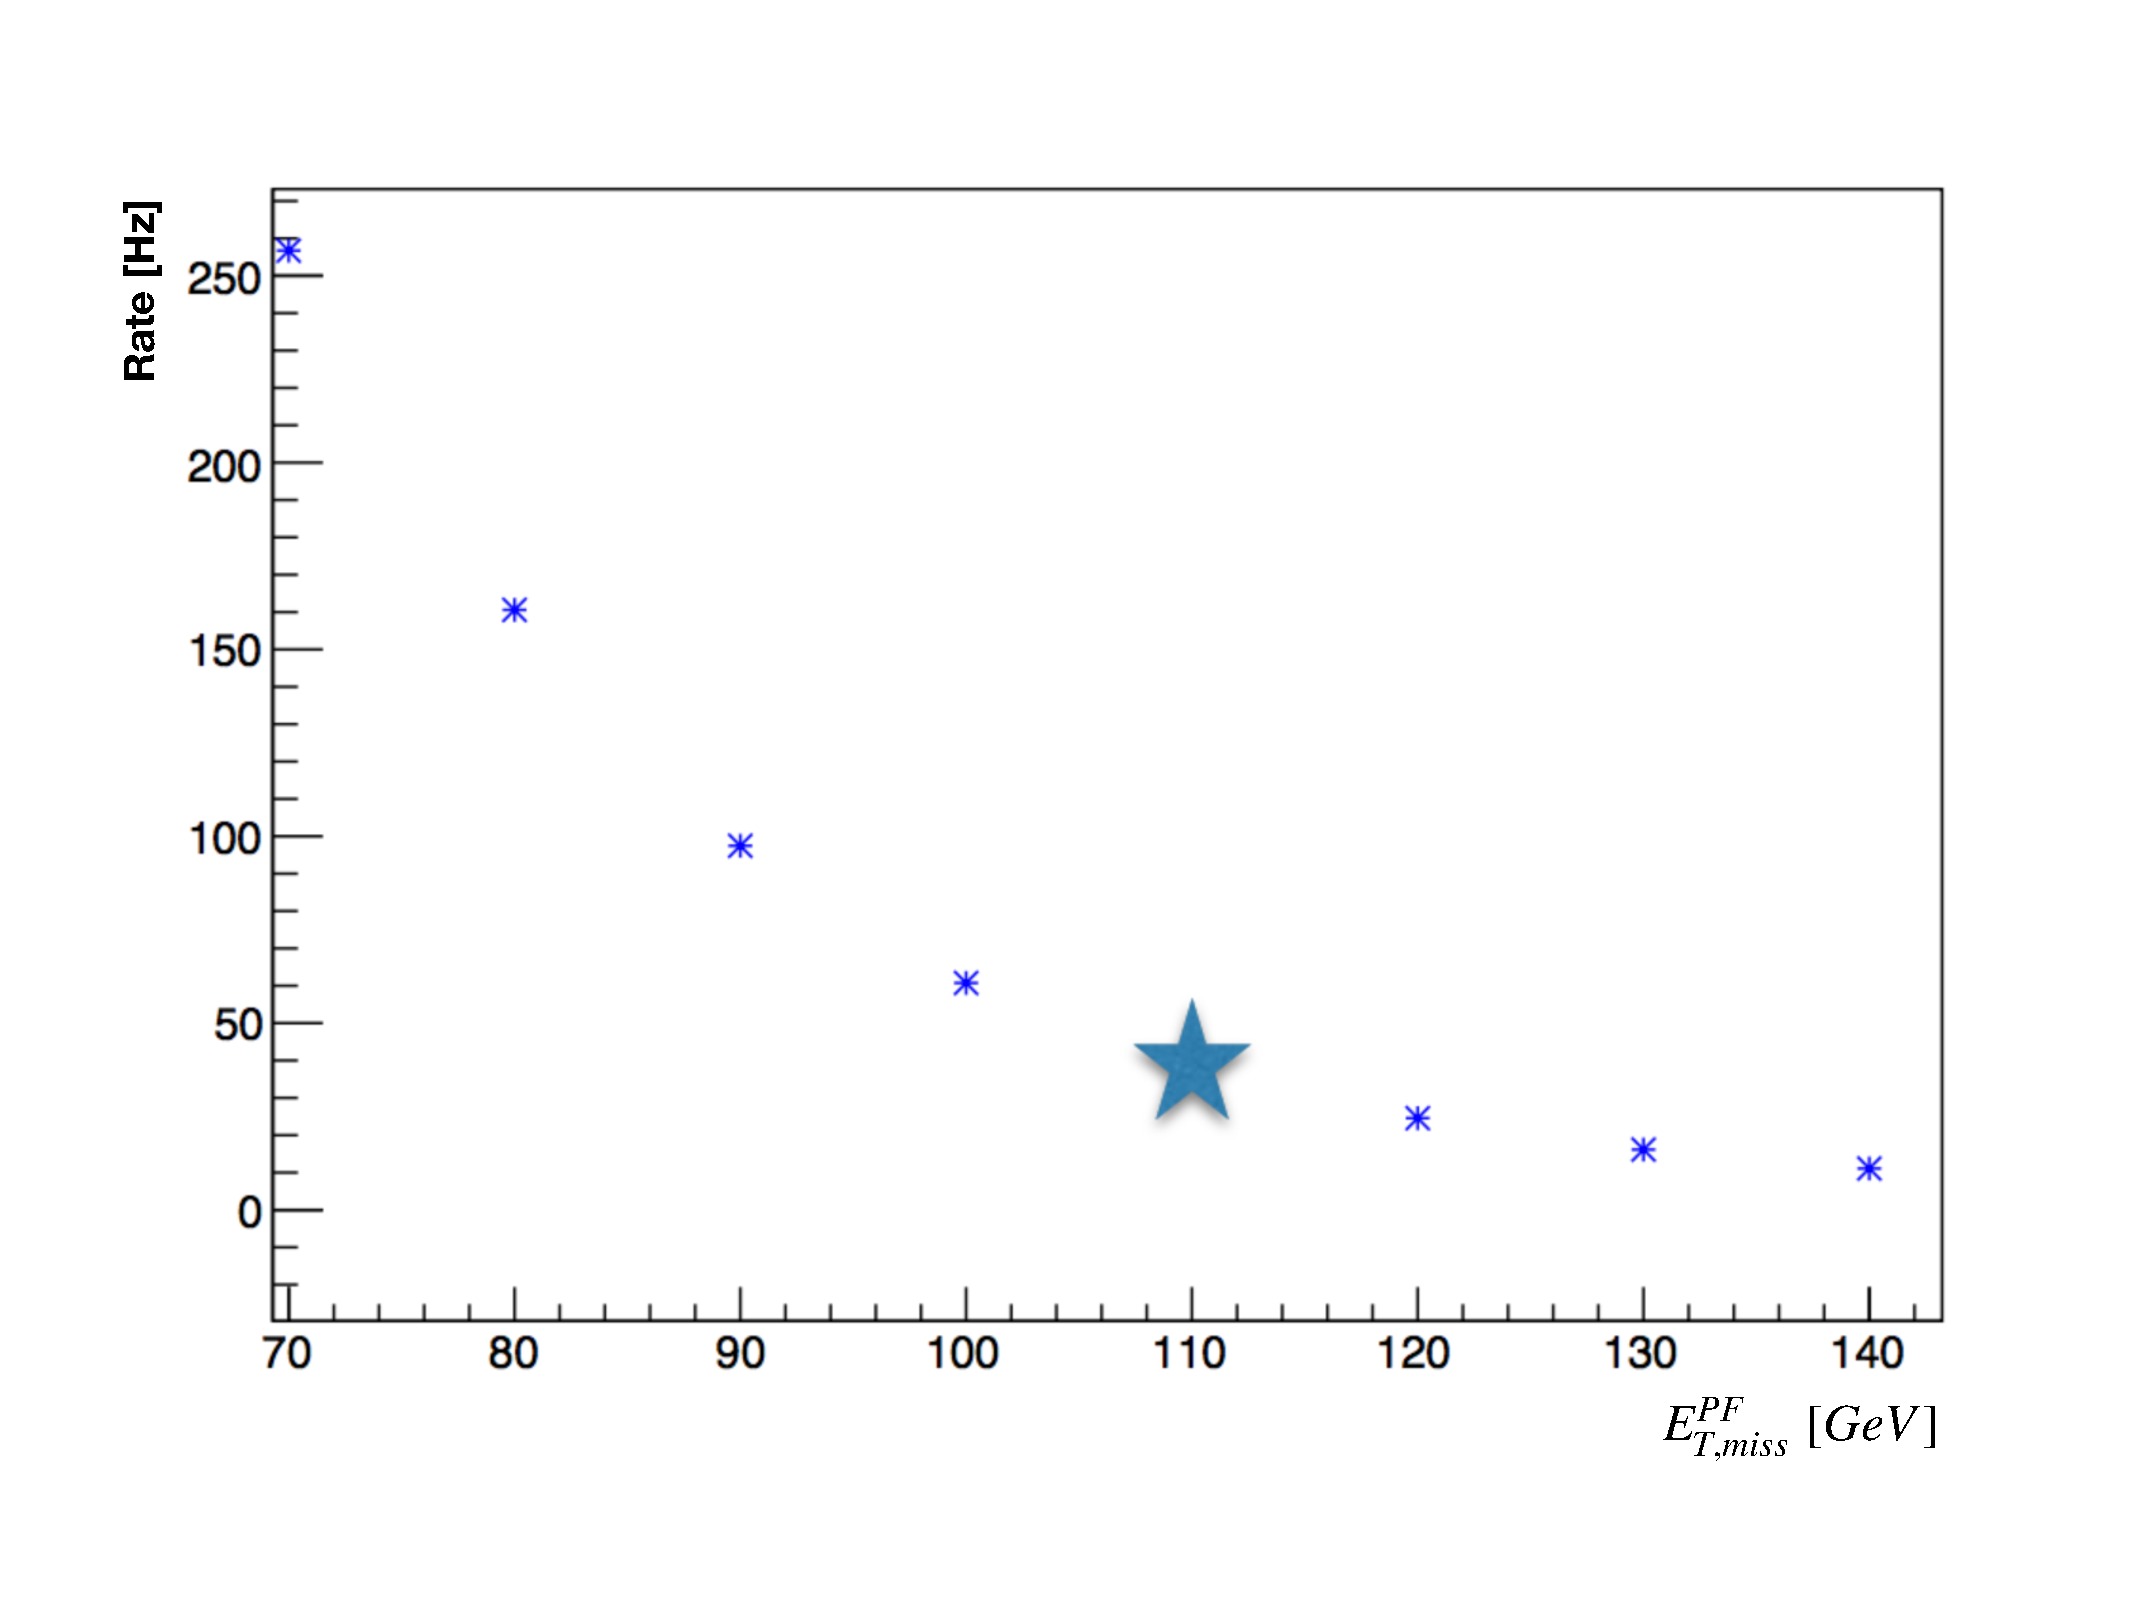
\includegraphics[width=0.75\textwidth]{CMS_experiment/PFMETvsRate.pdf}
  \caption{Estimate of the total rate of the dijet VBF HLT path versus the requirement on the $E_{T,miss}$.}
  \label{fig:PFMETvsRate}
\end{figure}
Potential issues that come with timing are directly related to the usage of the PF algorithm. As it requires the largest amount of time, a requirement was implemented in order to reduce the amount of events that would initialize it and then proceed to be rejected due to the $E^{PF}_{T,miss}>$~110~GeV requirement. This has lead to the inclusion of the $E^{Calo, NC}_{T,miss}$ selection listed above. A correlation study between these two $E_{T,miss}$ variables was performed (as shown in Figure~\ref{fig:VBF_rates_timing}). 
\begin{figure}[!htbp]
  \centering
    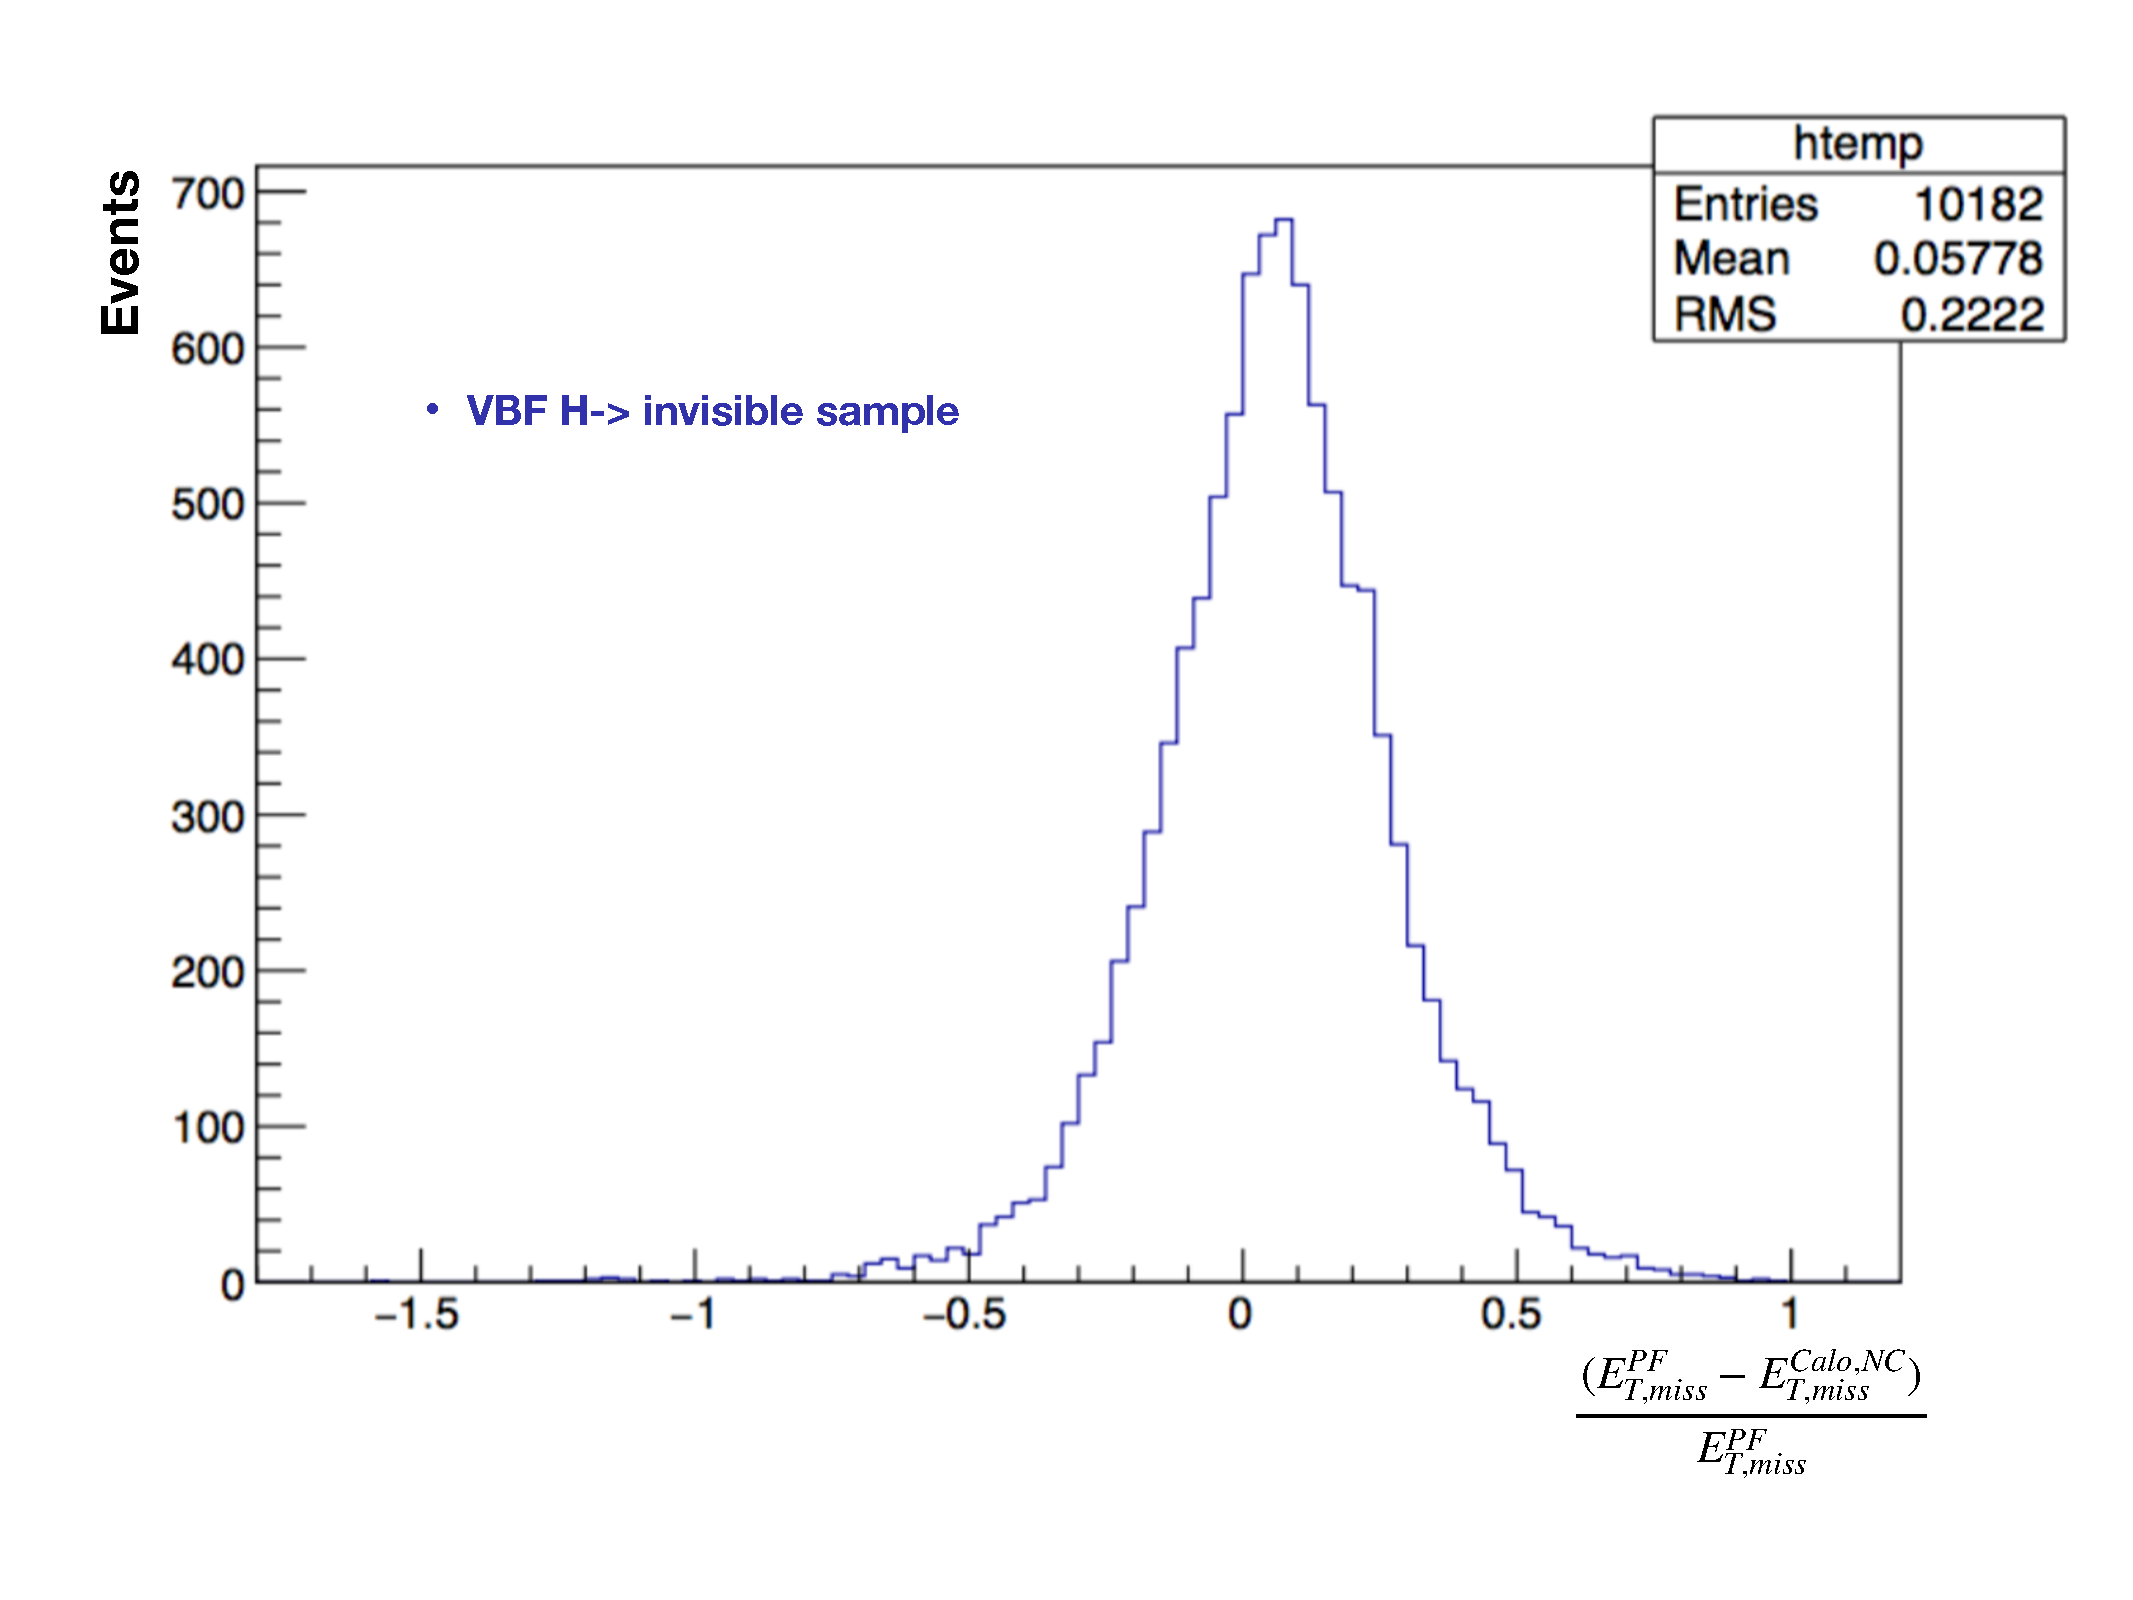
\includegraphics[width=0.75\textwidth]{CMS_experiment/PFvsCaloMET.pdf}
  \caption{Correlation study between the $E^{PF}_{T,miss}$ and $E^{Calo,NC}_{T,miss}$ done using the VBF H$\rightarrow$inv simulation sample.}
  \label{fig:VBF_rates_timing}
\end{figure}
It can be seen that no significant signal loss is expected if a requirement on the $E^{Calo, NC}_{T,miss}$ is imposed to be $\sim$60~\% of the one on the $E^{PF}_{T,miss}$. This, as a result, will stop a large amount of events from reaching modules which call the PF algorithm, instead stopping right after the $E^{Calo, NC}_{T,miss}$ producers, which take a lot less time.

\hspace{10pt} The triple jet path inherits most of the same workflow as its dijet counterpart, differing only in the final choice of jets. This triple jet category is more oriented towards analyses such as the VBF H$\rightarrow$bb$\tau\tau$, where it might bring additional sensitivity. From the perspective of the H$\rightarrow$ inv analysis, this triple jet scenario is valuable as a safeguard option for the subtle differences between the offline and HLT PF jets (which can also be seen by its significantly smaller rate).

\hspace{10pt} These HLT paths were introduced during the 2017 data collection and continued to be used in their original state until the end of the Run 2 phase. The pure and total rate of these paths for the 2018 data taking period are given in Table~\ref{tab:hlt_rates}. Their performance is going to be described in Section~\ref{subsec:vtr_selection}, where it will be shown how they influenced the creation of a new analysis subcategory.

\begin{table}[htbp]
    \centering
    \footnotesize
    \begin{tabular}{llcc}
     Path name & Status &Total Rate [Hz] & Pure Rate [Hz] \\   \hline\hline
           & & & \\
      HLT\_DiJet110\_35\_Mjj650\_PFMET110\_v*   &  signal & 36.88 & 7.84\\
      HLT\_DiJet110\_35\_Mjj650\_PFMET120\_v*   &  backup & 25.81 &  0 \\
      HLT\_DiJet110\_35\_Mjj650\_PFMET130\_v*   &  backup & 18.99 &  0\\
      & & &\\
      HLT\_TripleJet110\_35\_35\_Mjj650\_PFMET110\_v* & signal & 0.91 & 0.44 \\
      HLT\_TripleJet110\_35\_35\_Mjj650\_PFMET120\_v* & backup & 0.44 & 0\\
      HLT\_TripleJet110\_35\_35\_Mjj650\_PFMET130\_v* & backup & 0.25 & 0\\
      & & & \\\hline\hline
    \end{tabular}
    \caption{Measurement of rates for main VBF paths and their backups during 2018 era of data taking.}
    \label{tab:hlt_rates}
\end{table}

\hspace{10pt} As a final remark, it is important to note that even though the matching module had been created for the purposes of the VBF$\rightarrow$inv analysis, it has been used in other studies of the Higgs boson within the CMS experiment, such as the aforementioned $H\rightarrow \tau\tau /~ HH\rightarrow bb\tau\tau$ analyses, helping them to take the advantage of the L1 VBF seed by building their VBF HLT paths.

 



%\section{HLT performance during Run 2}
%\subsection{Introduction}
%\hspace{10pt} Being a general purpose detector, the CMS experiment has a range of dedicated working groups with each being in charge of a particular area of research. In order to efficiently illustrate the performance of the HLT during the Run 2 era, the following paragraphs are going to showcase selected examples of paths within the control of the Higgs Trigger Group. 
%\subsection{Performance of the cross triggers}
%\subsection{Performance of the VBF tau triggers}
%\subsection{Conclusion}


 \tikzset{
    pgfornamentstyle/.style={scale=0.4}
  }
\begin{center}
    \expandafter\pgfornament\expandafter{88}
\end{center}
 \tikzset{
    pgfornamentstyle/.style={scale=1}
  }
\restoregeometry